\documentclass{ieeeaccess}
\usepackage{cite}
\usepackage{amsmath,amssymb,amsfonts}
\usepackage{algorithmic}
\usepackage{algorithm}
\usepackage{graphicx}
\usepackage{textcomp}
\usepackage{booktabs}
\usepackage{multirow}
\usepackage{array}
\usepackage{url}
\usepackage{etoolbox}
\usepackage{tikz}
\usetikzlibrary{arrows.meta,positioning,fit,calc,backgrounds}
%% TikZ/xcolor breaks IEEE Access spot color --- restore blue title/ABSTRACT/sections
\definecolor{accessblue}{cmyk}{1,0.3,0,0.2}
\definecolor{greycolor}{cmyk}{0,0,0,0.8}
\usepackage{hyperref}
\hypersetup{
  colorlinks=true,
  linkcolor=blue,
  citecolor=blue,
  urlcolor=blue,
  breaklinks=true
}

\definecolor{cvL1}{RGB}{41,98,255}
\definecolor{cvL2}{RGB}{0,150,136}
\definecolor{cvL3}{RGB}{245,124,0}
\definecolor{cvL4}{RGB}{142,36,170}
\definecolor{cvL5}{RGB}{198,40,40}
\definecolor{cvJS}{RGB}{55,71,79}
\definecolor{cvSoft}{RGB}{236,239,241}
\definecolor{cvAdmin}{RGB}{25,118,210}
\definecolor{cvDash}{RGB}{67,160,71}

\makeatletter
\renewcommand{\headerlogo}{}
\renewcommand{\headerlogoall}{}
\makeatother

\makeatletter
\@ifundefined{xfigwd}{\newdimen\xfigwd}{}
\AtBeginEnvironment{figure}{\xfigwd=\columnwidth}
\AtBeginEnvironment{table}{\xfigwd=\columnwidth}
\AtBeginEnvironment{figure*}{\xfigwd=\textwidth}
\AtBeginEnvironment{table*}{\xfigwd=\textwidth}
\AtBeginEnvironment{algorithm}{\xfigwd=\columnwidth}
\makeatother

\setcounter{secnumdepth}{2}
\renewcommand{\thesection}{\Roman{section}}
\renewcommand{\thesubsection}{\Alph{subsection}}

\def\BibTeX{{\rm B\kern-.05em{\sc i\kern-.025em b}\kern-.08em
    T\kern-.1667em\lower.7ex\hbox{E}\kern-.125emX}}

\begin{document}

%\history{}


\title{CyberVault: A Hybrid UEBA--ML--Deep Learning Framework with Multi-Objective Response Optimization for Real-Time Privileged Access Management (PAM)}

\author{\uppercase{Oumaima Alfairam}\authorrefmark{1},
\uppercase{Khalid El Yassini}\authorrefmark{1},
and \uppercase{Kenza Oufaska}\authorrefmark{2}}

\address[1]{IAOR Research Team, IA Laboratory, Moulay Ismail University, Meknes, Morocco}
\address[2]{LERMA Laboratory, International University of Rabat, Morocco}

\markboth{\MakeLowercase{\textit{IEEE Access}}}{ALFAIRAM \MakeLowercase{\textit{et al.}}: CyberVault for Real-Time PAM}

\corresp{
E-mail: o.alfairam@edu.umi.ac.ma, khalid.elyassini@gmail.com, kenza.oufaska@uir.ac.ma.}

\begin{abstract}
Privileged accounts are still among the most impactful targets for security compromises, even though many PAM tools do not analyze the behavior of recorded sessions. The paper describes CyberVault, an open-source analytical layer for JumpServer, which solves this problem. CyberVault uses five components including telemetry gathering, relational profiling, hybrid detection, explainable AI and multi-goal response optimization. The detection combines experts’ rules, UEBA baselines, tabular machine learning (Isolation Forest and Random Forest), sequence-based deep models (LSTM and optional Transformer) and privilege graph neural network. The pipeline is defined with definite values of risk metrics rR, rB, rM, rS and rG, max-fusion and the two objectives include usage of privileges within 2 objectives: incident response and privilege assignment. The tabular hybrid works on reproducible synthetic dataset (1,000 records, seed 42, split 70/30) and obtains F1=66.2\% and recall=82.0\% compared to F1 of the rule alone of 51.2\% (+29.3\% gain) with the latency of ~180 ms. The development of the five-command insider chain chosen for testing was detected by the sequence model with rS exceeding 0.94. The results of tests in Docker indicated that webhook is delivered and the critical commands are locked.

\end{abstract}

\begin{keywords}
Anomaly detection, deep learning, explainable artificial intelligence, graph neural networks, insider threat, multi-objective optimization, privileged access management, user and entity behavior analytics, Zero Trust.
\end{keywords}

\maketitle

\section{INTRODUCTION}
\label{sec:intro}

\IEEEPARstart{I}{n} March 2024, a European energy provider disclosed that an attacker had spent eleven days inside production systems using a valid bastion account. Session recordings existed. So did access approvals. What the company lacked was a mechanism to judge, in the minutes after \texttt{chmod 777 /etc/shadow}, whether that judgment should become an alert, a locked session, or an explained incident ticket. The breach did not fail on identity; it failed on \textit{privileged behavior analytics} during live access.

Stories of this kind are no longer edge cases. Verizon's incident data consistently show privilege misuse and credential abuse among the costliest attack paths~\cite{ref21}. At the same time, Zero Trust adoption pushes organizations to verify every session continuously, not only at login~\cite{ref4,ref22}. Privileged Access Management (PAM) answered the first generation of this problem: vault the password, broker the session, record the screen, satisfy the auditor~\cite{ref1,ref5}. The next generation is harder. Security teams now ask whether PAM can \textit{reason} about privileged behavior while the session is still open.

The economic stakes are concrete. A single compromised domain-admin session can propagate ransomware across hundreds of hosts before EDR correlation catches up. Mean time to detect (MTTD) for insider-like privilege abuse still measures in days in many SOCs~\cite{ref6,ref24}, while mean time to contain (MTTC) for a live bastion session could be seconds if the PAM plane itself enforces policy. CyberVault targets that asymmetry: treat the bastion webhook stream as a first-class analytics source, not an archival afterthought.

\subsection{CONTEXT}
Three forces shape this question. First, insider and insider-like attacks rose with remote administration and cloud consoles; the attacker often looks like a legitimate administrator~\cite{ref6}. Second, privileged accounts remain disproportionately valuable---a single \texttt{root} session on a payment cluster can dwarf thousands of phishing attempts. Third, regulatory frameworks (NIS2, DORA, ISO~27001) expect both preventive controls and demonstrable monitoring. Commercial PAM suites---CyberArk, BeyondTrust, Delinea---matured on vaulting, Just-In-Time (JIT) access, and session isolation~\cite{ref16,ref17,ref18}. Open-source JumpServer~\cite{ref5} democratized bastion deployment but, in its default form, still behaves like a capable recorder rather than an analytic decision system.

From a research angle, the gap sits between two mature lines of work. Insider-threat studies (CERT, LANL, CMU) train offline classifiers on historical logs~\cite{ref10,ref24}. PAM engineering focuses on session reliability and credential hygiene~\cite{ref1,ref26}. CyberVault connects them through an online webhook contract: each command becomes a feature vector, and each response is the outcome of a constrained optimization. The MRQ is therefore not ``which classifier wins in isolation,'' but whether an integrated pipeline changes SOC outcomes on a bastion that is already in production.

\subsection{PROBLEM STATEMENT}
Field deployments reveal four recurring gaps between recording and response.
\begin{itemize}
\item \textbf{Detection latency.} Destructive commands and off-hours lateral movement are often found in quarterly log reviews, not in the active session.
\item \textbf{Alert quality.} A single behavioral engine may either miss contextual abuse (rules-only recall 34.4\% in our tests) or flood analysts (UEBA-only false-positive rate 16.7\%).
\item \textbf{Analyst trust.} Machine-learning scores without feature-level explanation are frequently ignored~\cite{ref12,ref13}.
\item \textbf{Response rigidity.} Static thresholds treat a maintenance window and a suspected breach identically; they do not optimize trade-offs between security, disruption, and alert fatigue~\cite{ref14,ref15}.
\end{itemize}
CyberVault was built to close these gaps on JumpServer without replacing it: webhook in, scored decision out, optional lock/kill when policy allows.

\subsection{MAIN RESEARCH QUESTION AND SUB-QUESTIONS}
The \textbf{main research question (MRQ)} that guides this study is:
\begin{quote}
\textit{How can an integrated artificial-intelligence, explainable-AI, and operations-research framework improve real-time detection, explanation, and response optimization for privileged-access sessions on open-source PAM?}
\end{quote}
We decompose the MRQ into four \textbf{sub-research questions (SRQs)}:
\begin{itemize}
\item \textbf{SRQ1 (Detection):} Can a hybrid ensemble (expert rules, behavioral UEBA, tabular ML, and deep sequence/graph scorers) detect privileged-account anomalies more effectively than any single engine on reproducible PAM telemetry?
\item \textbf{SRQ2 (Explainability):} Can SHAP and LIME attributions, combined with rule and UEBA textual reasons, make alerts actionable for SOC analysts during live sessions?
\item \textbf{SRQ3 (Optimization):} Can multi-objective response selection outperform static threshold policies when kill constraints and protected accounts bind?
\item \textbf{SRQ4 (Integration):} Does joint pipeline design produce measurable detection gain over sequential or isolated single-engine use?
\end{itemize}
Sections~\ref{sec:experiments}--\ref{sec:discussion} address SRQ1--SRQ4 with benchmark evidence and prototype measurements.

\subsection{CONTRIBUTIONS}
Four contributions follow from this design.
We first specify CyberVault as a five-layer intelligent-PAM stack on JumpServer---collect, profile, detect, explain, and decide---without replacing the bastion itself.
Second, we publish the full mathematical model: sets and parameters, detection equations for rules, UEBA, IF+RF, sequence score $r_S$, privilege GNN $r_G$, and the two MOO programs for privilege assignment~$(\mathrm{MO}\text{-}\mathrm{A})$ and incident response~$(\mathrm{MO})$/$(\mathrm{P})$.
Third, deep models run on the live path: a bidirectional LSTM (Transformer optional) over command history, plus a two-layer GNN over user--asset--IP relations, both trained offline and loaded at inference.
Fourth, we report reproducible numbers: tabular hybrid $F1=66.2\%$ (recall $82.0\%$, $n_{\mathrm{test}}=300$, seed~42), +29.3\% relative $\mathrm{Gap}_{F1}$ over rules-only, median latency near 180\,ms, and a five-command progressive case where tabular fusion stays at $r{=}0$ while $r_S\geq 0.94$.

The paper proceeds as follows. Section~\ref{sec:related} reviews related work; Section~\ref{sec:formulation} formalizes the model; Section~\ref{sec:framework} presents the architecture; Section~\ref{sec:implementation} covers the JumpServer prototype; Section~\ref{sec:method} describes methodology; Section~\ref{sec:experiments} reports results; Sections~\ref{sec:discussion}--\ref{sec:conclusion} discuss implications and conclude.

\section{LITERATURE REVIEW}
\label{sec:related}

\subsection{PRIVILEGED ACCESS MANAGEMENT}
PAM research and practice converged on least privilege, credential vaulting, session brokering, and tamper-evident audit~\cite{ref1,ref2,ref4,ref26}. Alruwies \textit{et al.}~\cite{ref1} propose an identity-governance framework for privileged users, while Tirtadjaja \textit{et al.}~\cite{ref2} address high-privileged account management in enterprise IT. In industry, CyberArk built its franchise on vault isolation and privileged session management for regulated enterprises~\cite{ref16}. BeyondTrust extended PAM toward endpoint privilege elevation and remote vendor access~\cite{ref17}. Delinea (formerly Thycotic/Centrify) concentrated on secret rotation and policy-based elevation~\cite{ref18}. JumpServer~\cite{ref5} occupies a different niche: open, self-hosted bastion with strong SSH/RDP/database proxying and recording, widely deployed where license cost matters.

Three PAM concepts recur in every vendor architecture and in our telemetry schema. \textbf{Least privilege} limits standing admin rights; JIT grants temporary elevation with approval workflows. \textbf{Session monitoring} records commands and video for audit. \textbf{Credential vault} removes shared passwords from tickets. Koot~\cite{ref26} introduces PAM concepts for interactive and non-interactive privileged accounts, including cloud-oriented use cases. What is less standardized is \textit{behavioral analytics on the session stream itself}---the point where CyberVault attaches.

These platforms excel at \textit{controlling entry}. They are weaker at \textit{judging behavior after entry}. Session monitoring produces rich telemetry---logins, commands, durations, assets, source IPs---yet native analytics remain limited compared with dedicated UEBA or SIEM correlation~\cite{ref27}. That asymmetry motivates an attachable AI layer rather than a rip-and-replace PAM migration.

\textbf{Comparative positioning.} Table~\ref{tab:pam-compare} contrasts capability emphasis. CyberVault does not replace vaulting; it augments open bastions where license cost or data-sovereignty rules preclude CyberArk-class suites.

\begin{table*}[!t]
\caption{PAM Platform Capability Emphasis}
\label{tab:pam-compare}
\centering
\scriptsize
\begin{tabular*}{\textwidth}{@{\extracolsep{\fill}}lcccc@{}}
\toprule
\textbf{Capability} & CyberArk & JumpServer & UEBA SIEM & CyberVault \\
\midrule
Credential vault & Strong & Partial & No & No \\
Session proxy & Strong & Strong & No & No \\
Live command stream & Yes & Yes & Delayed & Yes \\
Behavioral scoring & Add-on & Limited & Yes & Yes \\
Sequence / graph DL & Rare & No & Partial & Yes \\
XAI on session & Rare & No & Partial & Yes \\
MOO response & Playbooks & Manual & Playbooks & Yes \\
Open source & No & Yes & No & Yes \\
\bottomrule
\end{tabular*}
\end{table*}

\subsection{ZERO TRUST AND PAM CONVERGENCE}
NIST SP 800-207~\cite{ref22} defines Zero Trust as continuous verification, not a one-time gate. PAM is the practical enforcement arm for administrators: every SSH click passes through a policy point. NIS2 and ISO~27001~\cite{ref28,ref29} increasingly expect demonstrable monitoring, not checkbox vaulting. CyberVault operationalizes continuous verification by scoring each command event and optionally constraining the session before logout. This is not a replacement for network segmentation; it is the \textit{administrator-facing} slice of Zero Trust where blast radius is highest~\cite{ref21}.

\subsection{ANOMALY DETECTION FOR PRIVILEGED BEHAVIOR}
Insider-threat literature offers a spectrum of detectors~\cite{ref6,ref7,ref11,ref24,ref32,ref40,ref42,ref45}. Recent IEEE Access and Springer reviews synthesize classical ML, deep learning, and open challenges on CERT-style corpora~\cite{ref24,ref31,ref40,ref48}.

\textbf{Statistical approaches} such as $Z$-score thresholds and Mahalanobis distance flag multivariate outliers when baseline mean and covariance are stable~\cite{ref7}. They are interpretable---an analyst can see which dimension exceeded $\mu+3\sigma$---but brittle under concept drift. Admin teams rotate on-call weeks; a Mahalanobis model trained on January may declare March maintenance anomalous.

\textbf{Classical machine learning} includes One-Class SVM~\cite{ref20}, Local Outlier Factor~\cite{ref19}, and Isolation Forest (IF)~\cite{ref8}. LOF compares local density; it works well on clustered user groups but scales awkwardly on high-volume bastions. OCSVM finds a tight boundary around normal embeddings; tuning $\nu$ is non-trivial when attack prior is low. IF is attractive for PAM because it trains on predominantly normal sessions and scores isolation difficulty; CyberVault adopts IF with contamination $\pi=0.08$ on normal-only training data. In bastion telemetry, feature dimensionality stays modest ($|\mathcal{F}|=12$; see Section~\ref{sec:formulation}), which favors tree ensembles over deep embeddings for latency-sensitive paths~\cite{ref7,ref8}.

\textbf{Sequence and graph models.} Tuor \textit{et al.}~\cite{ref10} and Nasir \textit{et al.}~\cite{ref31} show that LSTM / deep autoencoders improve detection on CERT releases when enough compute is available; Transformer encoders~\cite{ref36} are an optional sequence backbone in CyberVault. Graph Neural Networks~\cite{ref23,ref37} treat users and assets as nodes with access edges; they help when relational structure matters. JumpServer webhooks already expose the triples $(u,a,i)$ and the ordered command stream $\mathcal{H}_s$ needed for both families. The practical question is not only offline AUC, but whether such models can run on the webhook path in well under a second and still cooperate with rules, UEBA, and MOO. Dataset portability follows CERT documentation~\cite{ref43}.

\textbf{Supervised ensembles} such as Random Forest (RF)~\cite{ref30} use labeled incidents when available~\cite{ref9,ref11}. In our benchmark, RF alone reached 100\% precision but only 22.9\% recall---accurate when it fires, silent when it does not. That asymmetry is why fusion matters: RF contributes precision; rules and UEBA contribute recall on complementary slices.

CyberVault therefore combines rules (signature certainty), UEBA (per-admin baselines), tree-based ML (IF+RF, SHAP-compatible), a sequence deep model for progressive command chains, and a lightweight privilege GNN for relational novelty, all under max-fusion and MOO constraints. LOF and OCSVM remain external baselines for future CERT/LANL ports (Section~\ref{sec:conclusion}).

\subsection{EXPLAINABLE ARTIFICIAL INTELLIGENCE}
Security operators distrust scores they cannot defend to a CIO. SHAP~\cite{ref12} attributes predictions to features via Shapley values; TreeExplainer makes this practical for Random Forests. LIME~\cite{ref13} fits a local linear surrogate around each event. Broader XAI-for-cybersecurity surveys motivate analyst-facing explanations~\cite{ref25}. Deep cybersecurity overviews situate neural detectors in the same stack~\cite{ref46}. For sequence models, CyberVault exposes token-stage hints (recon, pivot, exfil) alongside $r_S$; full attention-map visualization for the Transformer variant is left as medium-term work. CyberVault uses SHAP+LIME consensus with top-$k=5$ features on the RF path and falls back to RF importances when explainers timeout.

\subsection{OPERATIONS RESEARCH IN SECURITY RESPONSE}
Security orchestration often relies on playbooks with fixed ordering~\cite{ref15,ref41}. MOO scalarization instead minimizes a weighted sum of competing objectives subject to constraints---a pattern surveyed in engineering MOO~\cite{ref39} and used when Pareto front enumeration is too slow for online use~\cite{ref14,ref33,ref38}. Cyber-defence MOO on attack graphs~\cite{ref33}, Pareto-efficient response plans~\cite{ref38}, and AI-driven multi-objective mitigation engines~\cite{ref34} show that security, cost, and continuity can be optimized jointly. NSGA-II~\cite{ref35} remains the standard evolutionary alternative for offline Pareto exploration (future work). Khamlichi \textit{et al.}~\cite{ref14} showed that integrating lot-sizing with layout design beats sequential optimization by 6.34\% on average in manufacturing; we transpose that \textit{integration value} question to PAM: does fusing detection engines and OR-based response beat any isolated engine? Zero Trust companion guidance~\cite{ref22,ref47} frames continuous privileged verification as the policy backdrop.

\subsection{CHRONOLOGICAL EVOLUTION OF PAM ANALYTICS}
Understanding CyberVault's design requires a brief chronology. \textbf{Phase 1 (2005--2015):} PAM meant shared-password elimination and session recording; analytics, if any, were manual replay. CyberArk and BeyondTrust productized vaulting for Fortune~500 estates~\cite{ref16,ref17}. \textbf{Phase 2 (2015--2020):} JIT elevation and cloud bastions appeared; JumpServer~\cite{ref5} and similar open tools lowered deployment cost. UEBA vendors (Exabeam, Securonix) marketed standalone behavioral products fed by SIEM logs~\cite{ref2,ref27}. \textbf{Phase 3 (2020--present):} Zero Trust and NIS2~\cite{ref28,ref29} demand \textit{continuous} privileged verification; XAI and SOAR mature~\cite{ref12,ref13,ref15}; academic insider-threat benchmarks (CERT, LANL) push deep models~\cite{ref10,ref23}. Yet Phase~3 integrations remain fragmented: the bastion records, the UEBA correlates overnight, the SOAR playbook fires on tickets---not on the live \texttt{ssh} channel. CyberVault proposes a Phase~4 pattern: analytics and response \textit{on the webhook path} with a fully specified mathematical model.

\subsection{SCIENTIFIC GAP}
Most published systems are strong on one slice---detection, explanation, or response---but rarely close the loop on a live bastion webhook with equations that others can reproduce. Commercial UEBA add-ons seldom publish MOO constraints such as protected \texttt{root} accounts or a minimum kill confidence next to SHAP/LIME outputs. CERT and LANL studies push deep models further, yet they usually stop at classification rather than session lock. Hybrid surveys~\cite{ref11,ref24} argue for ensembles without a PAM-specific response model. Khamlichi \textit{et al.}~\cite{ref14} measured the value of integrating decisions in manufacturing; we ask the same kind of question for PAM engines and report $\mathrm{Gap}_{F1}$ explicitly on JumpServer.

\section{PROBLEM STATEMENT AND MODEL FORMULATION}
\label{sec:formulation}

The problem combines online detection, explanation, and constrained decisions over the event set $\mathcal{E}$. Notation and variables come first, then assumptions and detection equations. Response is written as two OR programs---privilege assignment and incident containment---each minimizing or maximizing an objective under feasibility constraints (Table~\ref{tab:moo-coexist}).

\subsection{NOTATIONS AND DECISION VARIABLES}

\textbf{1) SETS}

$\mathcal{E}=\{1,2,\ldots,E\}$ privileged-access events index

$\mathcal{U}=\{1,2,\ldots,U\}$ administrator identities index

$\mathcal{A}=\{1,2,\ldots,A\}$ protected assets index

$\mathcal{I}=\{1,2,\ldots,I\}$ source IP addresses index

$\mathcal{H}=\{0,1,\ldots,23\}$ hours-of-day index (UTC)

$\mathcal{J}=\{1,2,\ldots,J\}$ rule-family index ($J=4$ weight groups over multiple regex patterns)

$\mathcal{S}=\{1,2,\ldots,S\}$ UEBA behavioral-signal index ($S=8$)

$\mathcal{F}=\{1,2,\ldots,12\}$ machine-learning feature indices

$\mathcal{R}=\{1,2,\ldots,6\}$ \textbf{response-action} index set ($\mathcal{R}$ for \textit{response}; distinct from asset set $\mathcal{A}$)

$\mathcal{L}=\{1,2,\ldots,6\}$ \textbf{privilege-level} index set for access assignment (Table~\ref{tab:priv-moo})

$\mathcal{P}\subset\mathcal{U}$ kill-protected administrator accounts

\textbf{2) MODEL PARAMETERS}

$w_j$ : Rule weight for indicator $j\in\mathcal{J}$; $w_1=0.92$, $w_2=0.85$, $w_3=0.25$, $w_4=0.70$

$\delta_s$ : UEBA signal weight for $s\in\mathcal{S}$; Table~\ref{tab:ueba-signals}

$E_a$ : \textbf{E}xposure factor remaining if response $a\in\mathcal{R}$ is applied ($E_a\in[0,1]$); Table~\ref{tab:moo-costs}

$D_a$ : \textbf{D}isruption cost of response $a$ ($D_a\in[0,0.90]$); Table~\ref{tab:moo-costs}

$N_a$ : \textbf{N}otification load of response $a$ ($N_a\in[0,1]$); Table~\ref{tab:moo-costs}

$\lambda_1,\lambda_2,\lambda_3$ : Response-MOO weights on $F_1,F_2,F_3$ ($\lambda_1{=}0.55$, $\lambda_2{=}0.30$, $\lambda_3{=}0.15$)

$\mu_1,\mu_2,\mu_3$ : Privilege-MOO weights on $Z_1,Z_2,Z_3$ ($\mu_1{=}0.45$, $\mu_2{=}0.30$, $\mu_3{=}0.25$)

$\mathrm{Risk}_{\ell},\mathrm{Priv}_{\ell},\mathrm{Avail}_{\ell}$ : Cyber risk, privilege mass, and availability of level $\ell\in\mathcal{L}$ (Table~\ref{tab:priv-moo})

$\tau_a,\tau_l,\tau_k$ : Alert, lock, kill risk thresholds ($0.55$, $0.75$, $0.90$)

$\omega_{\mathrm{RF}}$ : RF blend weight ($\omega_{\mathrm{RF}}=0.60$)

$\rho_{\mathrm{learn}}$ : UEBA learning cap ($\rho_{\mathrm{learn}}=0.40$)

$\pi$ : IF contamination ($\pi=0.08$)

$n_{\mathrm{IF}},n_{\mathrm{RF}}$ : Tree counts ($200$ each)

$d_{\mathrm{RF}}$ : RF max depth ($12$)

$c_{\min}$ : Minimum kill confidence ($0.70$)

$\eta$ : Typical-hour threshold ($0.05$)

$\mathcal{H}_s$ : Ordered command history of session $s$, $\mathcal{H}_s=(c_1,\ldots,c_t)$

$T$ : Max tokens per command ($T{=}24$)

$L$ : Max commands in sequence window ($L{=}16$)

$\tau_{\mathrm{temp}}$ : Sequence score temperature ($\tau_{\mathrm{temp}}{=}1.5$)

$N_{\min}$ : Minimum events for UEBA scoring ($N_{\min}=5$)

$x_{fj}$ : Value of feature $j\in\mathcal{F}$ for event $e$

$y_e$ : Ground-truth label ($1$ anomaly, $0$ normal), offline only

\textbf{3) DECISION VARIABLES}

$x_a(e)$ : Binary selection of response $a\in\mathcal{R}$ for event $e$ ($x_a(e)\in\{0,1\}$)

$y_{\ell}(e)$ : Binary selection of privilege level $\ell\in\mathcal{L}$ for event/session $e$ ($y_{\ell}(e)\in\{0,1\}$)

$Z_1,Z_2,Z_3$ : Privilege-MOO objectives (risk, privilege mass, availability)

$F_1(x;e),F_2(x),F_3(x)$ : Response-MOO objectives (security, disruption, notification) to minimize

$Z(x;e)$ : Scalarized response objective $Z=\lambda_1 F_1+\lambda_2 F_2+\lambda_3 F_3$

$W(y;e)$ : Scalarized privilege objective (minimize form of~$(\mathrm{MO}\text{-}\mathrm{A})$)

$r_R(e)$ : Rules risk score, $r_R(e)\in[0,1]$

$r_B(e)$ : UEBA behavioral score, $r_B(e)\in[0,1]$

$r_M(e)$ : ML ensemble score, $r_M(e)\in[0,1]$

$r_S(e)$ : Sequence DL score (LSTM/Transformer), $r_S(e)\in[0,1]$

$r_G(e)$ : Privilege GNN score, $r_G(e)\in[0,1]$

$r(e)$ : Fused hybrid risk score, $r(e)\in[0,1]$

$c(e)$ : Fused confidence, $c(e)\in[0,1]$

$a^*(e)$ : Selected response action, $a^*(e)\in\mathcal{R}$

$\phi_j(e)$ : SHAP attribution for feature $j$

$z_j(e)$ : Binary rule trigger ($1$ if rule $j$ fires)

$v_s(e)$ : Binary UEBA signal trigger ($1$ if signal $s$ fires)

$b_u$ : Behavioral baseline of administrator $u$
\begin{table}[!t]
\caption{UEBA Signal Weights $\delta_s$}
\label{tab:ueba-signals}
\centering
\footnotesize
\begin{tabular}{lc|lc}
\toprule
\textbf{Signal} $s$ & $\delta_s$ & \textbf{Signal} $s$ & $\delta_s$ \\
\midrule
Unusual hour & 0.50 & Login failed & 0.55 \\
Unusual asset & 0.55 & Failed burst ($\geq 3$) & 0.70 \\
Unusual IP & 0.55 & Lateral ($>4$ assets) & 0.65 \\
High velocity & 0.40 & Unusual account & 0.45 \\
\bottomrule
\end{tabular}
\end{table}

\begin{table}[!t]
\caption{ML Feature Vector $\mathbf{x}(e)$}
\label{tab:features}
\centering
\footnotesize
\begin{tabular}{cl}
\toprule
\textbf{$j$} & \textbf{Feature $x_{fj}$} \\
\midrule
1--3 & normalized hour, session command count, user command total \\
4--6 & ACL violation, destructive command, login failure \\
7--9 & new asset, new IP, unusual hour \\
10--12 & command velocity ratio, lateral breadth, unknown account \\
\bottomrule
\end{tabular}
\end{table}

\begin{table}[!t]
\caption{MOO Cost Parameters by Response Action $a\in\mathcal{R}$}
\label{tab:moo-costs}
\centering
\scriptsize
\begin{tabular}{@{}clccc@{}}
\toprule
$a$ & \textbf{Action} & $E_a$ & $D_a$ & $N_a$ \\
\midrule
1 & NO\_ACTION & 1.00 & 0.00 & 0.00 \\
2 & LOG\_ONLY & 0.90 & 0.10 & 0.20 \\
3 & ALERT\_ANALYST & 0.60 & 0.35 & 1.00 \\
4 & CREATE\_TICKET & 0.50 & 0.45 & 1.00 \\
5 & LOCK\_SESSION & 0.20 & 0.65 & 0.00 \\
6 & KILL\_SESSION & 0.05 & 0.90 & 0.00 \\
\bottomrule
\end{tabular}
\\[0.35em]
{\scriptsize $E_a$: exposure; $D_a$: disruption; $N_a$: notification.}
\end{table}

\begin{table}[!t]
\caption{Privilege-Assignment MOO Coefficients by Level $\ell\in\mathcal{L}$}
\label{tab:priv-moo}
\centering
\scriptsize
\begin{tabular}{@{}clccc@{}}
\toprule
$\ell$ & \textbf{Privilege level} & $\mathrm{Risk}_{\ell}$ & $\mathrm{Priv}_{\ell}$ & $\mathrm{Avail}_{\ell}$ \\
\midrule
1 & DENY\_ACCESS & 0.05 & 0.00 & 0.10 \\
2 & READ\_ONLY & 0.15 & 0.20 & 0.85 \\
3 & STANDARD\_ADMIN & 0.35 & 0.45 & 0.95 \\
4 & JIT\_TIME\_LIMITED & 0.40 & 0.55 & 0.90 \\
5 & ELEVATED & 0.65 & 0.75 & 0.80 \\
6 & FULL\_ROOT & 0.95 & 1.00 & 0.70 \\
\bottomrule
\end{tabular}
\\[0.35em]
{\scriptsize $\mathrm{Risk}_{\ell}$: cyber risk if level granted; $\mathrm{Priv}_{\ell}$: privilege mass; $\mathrm{Avail}_{\ell}$: operational continuity.}
\end{table}

\begin{table}[!t]
\caption{Detection Components Deployed in CyberVault}
\label{tab:deployed-scope}
\centering
\scriptsize
\begin{tabular}{@{}ll c@{}}
\toprule
\textbf{Role} & \textbf{Engine} & \textbf{Status} \\
\midrule
Signature & Rules $r_R$ & Deployed \\
Behavioral & UEBA $r_B$ & Deployed \\
Tabular ML & IF+RF $\rightarrow r_M$ & Deployed \\
Sequence & LSTM/Transf.\ $r_S$ & Deployed \\
Privilege graph & GNN $r_G$ & Deployed \\
\bottomrule
\end{tabular}
\end{table}

\subsection{PROBLEM ASSUMPTIONS}
\begin{itemize}
\item Events arrive online via JumpServer webhook; median prototype latency is below 500\,ms on Docker v4.0.2.
\item UEBA scoring requires at least $N_{\min}=5$ prior events per user; baselines learn only when $r(e)\leq\rho_{\mathrm{learn}}=0.40$.
\item IF trains on normal labels only; RF uses balanced class weights on 700 training events; test fold has 300 events (seed 42).
\item Sequence DL and GNN train offline on labeled sessions (including progressive multi-step attack chains and hard-negative benign sessions); inference loads the serialized sequence and GNN model weights.
\item MOO weights $(\lambda_1,\lambda_2,\lambda_3)=(0.55,0.30,0.15)$ on response objectives $(F_1,F_2,F_3)$ and cost table $(E_a,D_a,N_a)$ are fixed policy constants (Table~\ref{tab:moo-costs}). Privilege-MOO weights $(\mu_1,\mu_2,\mu_3)=(0.45,0.30,0.25)$ and coefficients $(\mathrm{Risk}_{\ell},\mathrm{Priv}_{\ell},\mathrm{Avail}_{\ell})$ are fixed (Table~\ref{tab:priv-moo}).
\item Accounts in $\mathcal{P}=\{\texttt{root},\texttt{administrator}\}$ are kill-protected; kill requires $c(e)\geq 0.70$.
\item Corporate CIDRs 10.0.0.0/8 and 192.168.0.0/16 are UEBA-whitelisted.
\end{itemize}


\subsection{DESIGN TARGET, IMPLEMENTATION SCOPE, AND DETECTION MODELS}

\textbf{Long-term design target.} The literature often posits a weighted fusion of structural, temporal, and local anomaly scores:
\begin{equation}
A_i = w_1\,\mathrm{GNN}_i + w_2\,\mathrm{Transformer}_i + w_3\,\mathrm{IF}_i.
\tag{0}
\end{equation}
Equation~(0) is a conceptual target. CyberVault realizes that idea in practice through the engines in Table~\ref{tab:deployed-scope}: rules for signatures, UEBA and a privilege GNN for structure, an LSTM/Transformer for command sequences, and IF+RF for tabular local anomalies. Online fusion uses a conservative maximum (Equation~(4)) rather than fixed weights $w_1,w_2,w_3$, which keeps any high-confidence hit from being diluted.

\textbf{Expert rule model (deployed).} Let $z_j(e)\in\{0,1\}$ indicate whether rule $j\in\mathcal{J}$ matches event $e$ (destructive command regex, ACL violation, or high session velocity). The rule risk score is
\begin{equation}
r_R(e)=\min\!\left(1,\max_{j\in\mathcal{J}} w_j\, z_j(e)\right).
\tag{1}
\end{equation}
When no rule fires, $r_R(e)=0$. This is a deterministic expert system, not a learned model.

\textbf{UEBA behavioral model (deployed).} Each administrator $u\in\mathcal{U}$ maintains a baseline $b_u$ recording typical hours, assets, accounts, source IPs, and command velocities observed under normal activity. Let $v_s(e)\in\{0,1\}$ denote whether behavioral signal $s\in\mathcal{S}$ is active (e.g., unusual hour, new asset, lateral movement). If the baseline has at least $N_{\min}$ events, the behavioral score is
\begin{equation}
r_B(e)=\min\!\left(1,\max_{s\in\mathcal{S}} \delta_s\, v_s(e)\right);
\tag{2}
\end{equation}
otherwise $r_B(e)=0$ until the baseline warms up. Baseline update follows constraint~(10): $b_u$ is updated only when $r(e)\leq\rho_{\mathrm{learn}}$, preventing poisoning by attack traffic.

\textbf{Machine-learning ensemble (deployed).} Each event is mapped to $\mathbf{x}(e)=(x_{f1},\ldots,x_{f12})$ as in Table~\ref{tab:features}. The \textit{Isolation Forest} (IF) trains on normal-only samples ($y_e=0$) with $n_{\mathrm{IF}}$ trees and contamination $\pi$. Let $\mathrm{IF}(\mathbf{x})$ denote the Isolation Forest isolation score (negative decision function). After min--max calibration on training normals, the IF risk is
\begin{equation}
r_M^{\mathrm{IF}}(e) = \mathrm{clip}_{[0,1]}\!\left(\frac{-\mathrm{IF}(\mathbf{x}(e))-s_{\min}}{s_{\max}-s_{\min}}\right).
\tag{3.1}
\end{equation}
The \textit{Random Forest} (RF) classifier with $n_{\mathrm{RF}}$ trees and maximum depth $d_{\mathrm{RF}}$ estimates the posterior anomaly probability
\begin{equation}
r_M^{\mathrm{RF}}(e) = P(y{=}1\mid \mathbf{x}(e)) = \frac{1}{n_{\mathrm{RF}}}\sum_{t=1}^{n_{\mathrm{RF}}} \mathbb{1}\bigl[h_t(\mathbf{x}(e)){=}1\bigr],
\tag{3.2}
\end{equation}
where $h_t$ is the $t$-th tree and class labels are balanced during training. The deployed ML score blends both models:
\begin{equation}
r_M(e) = \omega_{\mathrm{RF}}\, r_M^{\mathrm{RF}}(e) + (1-\omega_{\mathrm{RF}})\, r_M^{\mathrm{IF}}(e).
\tag{3.3}
\end{equation}
If models are untrained, $r_M(e)=0$ and the hybrid pipeline relies on $r_R$ and $r_B$ (and deep scorers if present) only---a behavior observed during live warm-up.

\textbf{Sequence deep-learning model (deployed).}
Tabular engines score each event in isolation. Progressive insider attacks often keep every individual command plausible (no \texttt{rm -rf}, familiar IP, business hours) while the \textit{ordered} chain is malicious. Let $\mathcal{H}_s=(c_1,\ldots,c_t)$ be the session history available after enrichment (Layer~1 stores up to 50 commands; the encoder uses the last $L{=}16$). Each command $c_\ell$ is tokenized into at most $T{=}24$ tokens and embedded. Mean-pooled token embeddings yield a command vector; a bidirectional LSTM (default) or Transformer encoder (optional policy switch) maps the command sequence to a raw probability $\tilde{r}_S(e)\in(0,1)$. Temperature calibration softens overconfidence:
\begin{equation}
r_S(e)=\sigma\!\left(\frac{\mathrm{logit}(\tilde{r}_S(e))}{\tau_{\mathrm{temp}}}\right),
\quad \tau_{\mathrm{temp}}=1.5.
\tag{3.4}
\end{equation}
Training minimizes weighted binary cross-entropy on session prefixes built from labeled events. Positive examples include progressive MITRE-style chains (recon $\rightarrow$ staging $\rightarrow$ pivot $\rightarrow$ lateral copy $\rightarrow$ archive+upload). Hard negatives include benign sessions that contain isolated \texttt{find}, \texttt{ssh}, or \texttt{curl} commands so the model must learn \textit{order}, not single tokens. Trained weights and the command vocabulary are persisted for online loading.

\textbf{Privilege GNN (deployed).}
Complementing UEBA baselines, we build an undirected heterogeneous privilege graph $G=(V,E)$ with node types user, asset, and IP. Training events add edges $(u,a)$, $(u,i)$, and $(a,i)$. A two-layer message-passing network produces node embeddings $h_v$. For event $e$ with triple $(u,a,i)$,
\begin{equation}
r_G(e)=\sigma\!\bigl(W[h_u\,\|\,h_a\,\|\,h_i]\bigr),
\tag{3.5}
\end{equation}
where $\|\,$ denotes concatenation. Unseen nodes map to dedicated unknown embeddings. Trained weights and the graph index are persisted for online loading. On the progressive Case~A chain (familiar user, asset, and IP), $r_G$ stays low---as expected---while $r_S$ carries detection; $r_G$ contributes when relational novelty appears.

\textbf{Hybrid fusion (deployed).} Detection engines run in parallel; fusion is conservative:
\begin{equation}
r(e)=\max\bigl(r_R(e),r_B(e),r_M(e),r_S(e),r_G(e)\bigr), \quad
c(e)=\max\bigl(c_R,c_B,c_M,c_S,c_G\bigr).
\tag{4}
\end{equation}
Max-fusion ensures that a high-confidence rule, behavioral, tabular-ML, sequence, or GNN hit is never averaged away---a design choice appropriate for privileged admin channels. Offline training versus online inference is summarized in Table~\ref{tab:train-infer}.

\begin{table}[!t]
\caption{Offline Training vs.\ Online Inference}
\label{tab:train-infer}
\centering
\scriptsize
\begin{tabular}{@{}l p{0.28\columnwidth} p{0.32\columnwidth}@{}}
\toprule
\textbf{Engine} & \textbf{Offline} & \textbf{Online} \\
\midrule
Rules $r_R$ & Configure regex/weights & Match command \\
UEBA $r_B$ & Warm baseline & Compare / learn if $r\leq 0.40$ \\
IF+RF $r_M$ & Fit on labeled $\mathbf{x}(e)$ & Score feature vector \\
Seq.\ $r_S$ & Train LSTM/Transformer & Score $\mathcal{H}_s$ \\
GNN $r_G$ & Train privilege graph & Score $(u,a,i)$ \\
MOO & Policy costs/weights & Privilege~$(\mathrm{MO}\text{-}\mathrm{A})$ then response~$(\mathrm{P})$ \\
\bottomrule
\end{tabular}
\end{table}

\subsection{DUAL MULTI-OBJECTIVE OPTIMIZATION}
Every privileged session forces two decisions that look similar on paper but are not the same problem.

The first is about access power: should the administrator stay read-only, receive time-limited JIT elevation, keep full root, or be denied? Too much privilege raises cyber risk; too little blocks legitimate work. We call this privilege assignment~$(\mathrm{MO}\text{-}\mathrm{A})$.

The second is about containment once detectors fire: leave the session alone, log quietly, page the SOC, lock, or kill. Stronger actions cut residual exposure but disturb operators and can flood the ticket queue. That is incident response~$(\mathrm{MO})$/$(\mathrm{P})$.

Privilege assignment shapes what the session is allowed to do; response reacts when fused risk $r(e)$ rises. Both are written as classical OR programs---minimize or maximize an objective subject to hard constraints---and both run on the same event. Table~\ref{tab:moo-coexist} contrasts them.

\begin{table}[!t]
\caption{Coexistence of the Two CyberVault MOO Programs}
\label{tab:moo-coexist}
\centering
\scriptsize
\begin{tabular}{@{}p{0.18\columnwidth} p{0.36\columnwidth} p{0.36\columnwidth}@{}}
\toprule
 & \textbf{$(\mathrm{MO}\text{-}\mathrm{A})$ Privilege assignment} & \textbf{$(\mathrm{MO})$/$(\mathrm{P})$ Incident response} \\
\midrule
\textbf{Question} & How much privilege to grant or keep? & How to contain a risky session? \\
\textbf{When} & Access / elevation / ongoing grant & After detection raises $r(e)$ \\
\textbf{Decision} & One privilege level $\ell^*\in\mathcal{L}$ & One session action $a^*\in\mathcal{R}$ \\
\textbf{Examples} & READ\_ONLY, JIT, FULL\_ROOT, DENY & LOG, ALERT, LOCK, KILL \\
\textbf{Objectives} & min cyber risk $Z_1$; min privilege mass $Z_2$; \textbf{max} continuity $Z_3$ & min residual exposure $F_1$; min disruption $F_2$; min alert load $F_3$ \\
\textbf{Online form} & Minimize $W=\mu_1 Z_1+\mu_2 Z_2+\mu_3(1-Z_3)$ & Minimize $Z=\lambda_1 F_1+\lambda_2 F_2+\lambda_3 F_3$ \\
\textbf{Hard constraints} & Forbidden levels; no FULL\_ROOT if $r(e)$ is very high & Protected accounts; kill only if confidence $\geq c_{\min}$ \\
\bottomrule
\end{tabular}
\end{table}

Consider an on-call engineer who needs elevated access at 02:00. Model~$(\mathrm{MO}\text{-}\mathrm{A})$ may grant \texttt{JIT\_TIME\_LIMITED} instead of standing \texttt{FULL\_ROOT}. If that session later issues a destructive command and $r(e)$ jumps, model~$(\mathrm{P})$ can still lock or kill without undoing the earlier least-privilege choice. Each event therefore returns both $\ell^*$ and $a^*$.

\subsection{PRIVILEGE-ASSIGNMENT MODEL $(\mathrm{MO}\text{-}\mathrm{A})$}

We want to choose the smallest useful privilege for the job: \textbf{minimize} cyber risk, \textbf{minimize} the amount of privilege granted, and \textbf{maximize} operational continuity, \textbf{subject to} choosing exactly one level and respecting policy bans.

Given a session or elevation request $e$, we select exactly one privilege level $\ell\in\mathcal{L}$ (Table~\ref{tab:priv-moo}). Decision variables:
\begin{equation}
y_{\ell}(e)\in\{0,1\}, \qquad \ell\in\mathcal{L}.
\tag{4.5}
\end{equation}

\textbf{Objective 1 --- Minimize cyber risk:}
\begin{equation}
\min\; Z_1(y;e)=\sum_{\ell\in\mathcal{L}} \mathrm{Risk}_{\ell}\, y_{\ell}(e).
\tag{A1}
\end{equation}

\textbf{Objective 2 --- Minimize granted privileges:}
\begin{equation}
\min\; Z_2(y;e)=\sum_{\ell\in\mathcal{L}} \mathrm{Priv}_{\ell}\, y_{\ell}(e).
\tag{A2}
\end{equation}

\textbf{Objective 3 --- Maximize operational continuity:}
\begin{equation}
\max\; Z_3(y;e)=\sum_{\ell\in\mathcal{L}} \mathrm{Avail}_{\ell}\, y_{\ell}(e).
\tag{A3}
\end{equation}

\textbf{Classical multi-objective model $(\mathrm{MO}\text{-}\mathrm{A})$.}
\begin{equation}
\begin{aligned}
(\mathrm{MO}\text{-}\mathrm{A})\quad
& \textbf{Minimize}\quad Z_1=\sum_{\ell\in\mathcal{L}} \mathrm{Risk}_{\ell}\, y_{\ell}(e) \\
& \textbf{Minimize}\quad Z_2=\sum_{\ell\in\mathcal{L}} \mathrm{Priv}_{\ell}\, y_{\ell}(e) \\
& \textbf{Maximize}\quad Z_3=\sum_{\ell\in\mathcal{L}} \mathrm{Avail}_{\ell}\, y_{\ell}(e) \\[0.35em]
& \textbf{subject to} \\
& \sum_{\ell\in\mathcal{L}} y_{\ell}(e)=1, \\
& y_{\ell}(e)\in\{0,1\},\ \forall \ell\in\mathcal{L}, \\
& y_{\mathrm{FULL\_ROOT}}(e)=0\ \text{if } r(e)\geq \tau_k, \\
& y_{\ell}(e)=0\ \text{if level $\ell$ is policy-forbidden for $u(e)$}.
\end{aligned}
\tag{A}\label{eq:moo-priv}
\end{equation}
In words: we never grant two levels at once; we never grant a level the policy forbids; and we refuse unrestricted root when fused risk is already at kill level. The three goals conflict---DENY or READ\_ONLY lowers $Z_1$ and $Z_2$ but also lowers continuity $Z_3$. For online use we rewrite maximization of $Z_3$ as minimization of $1-Z_3$ and scalarize:
\begin{equation}
\begin{aligned}
(\mathrm{P}\text{-}\mathrm{A})\quad
& \textbf{Minimize}\quad W(y;e)=\mu_1 Z_1+\mu_2 Z_2+\mu_3\bigl(1-Z_3\bigr) \\[0.35em]
& \textbf{subject to the same constraints as }(\mathrm{MO}\text{-}\mathrm{A}).
\end{aligned}
\tag{PA}\label{eq:moo-priv-scalar}
\end{equation}
Equivalently,
\begin{equation}
\ell^*(e)=\arg\min_{\ell\in\mathcal{L}'(e)}\bigl(\mu_1\mathrm{Risk}_{\ell}+\mu_2\mathrm{Priv}_{\ell}+\mu_3(1-\mathrm{Avail}_{\ell})\bigr),
\tag{A4}
\end{equation}
where $\mathcal{L}'(e)$ is the feasible privilege set after policy filters. Deployed weights: $\mu_1{=}0.45$, $\mu_2{=}0.30$, $\mu_3{=}0.25$.

\subsection{MULTI-OBJECTIVE RESPONSE OPTIMIZATION MODEL $(\mathrm{MO})$/$(\mathrm{P})$}

After detection and fusion (Equation~(4)), each event $e\in\mathcal{E}$ has a fused risk $r(e)\in[0,1]$ and a confidence $c(e)\in[0,1]$. Independently of which privilege level was granted, we must now answer: \textit{should we leave the session alone, warn someone, lock it, or kill it?} We want to \textbf{minimize} residual security exposure, operator disruption, and SOC notification load, \textbf{subject to} choosing exactly one action and respecting kill-governance rules~\cite{ref14,ref15}.

\textbf{1) Decision variables.}
\begin{equation}
x_a(e)\in\{0,1\}, \qquad a\in\mathcal{R},
\tag{5.0}
\end{equation}
where $x_a(e)=1$ if action $a$ is selected for event $e$, and $0$ otherwise.

\textbf{2) The three objectives.}
\begin{itemize}
\item $F_1$ --- \textbf{Security}: residual exposure left by the chosen action.
\item $F_2$ --- \textbf{Disruption}: disturbance imposed on the administrator.
\item $F_3$ --- \textbf{Notification}: alert/ticket load imposed on the SOC.
\end{itemize}
Using cost parameters $(E_a,D_a,N_a)$ from Table~\ref{tab:moo-costs}:
\begin{align}
F_1(x;e)
&=
\sum_{a\in\mathcal{R}} r(e)\, E_a\, x_a(e),
\tag{5.1}\\
F_2(x)
&=
\sum_{a\in\mathcal{R}} D_a\, x_a(e),
\tag{5.2}\\
F_3(x)
&=
\sum_{a\in\mathcal{R}} N_a\, x_a(e).
\tag{5.3}
\end{align}
Since exactly one $x_a$ equals 1, these reduce to $F_1=r(e)E_a$, $F_2=D_a$, $F_3=N_a$ for the chosen action. Reading the objectives in human terms:
\begin{itemize}
\item ignoring a high-risk event (large $E_a$) leaves too much exposure---$F_1$ is large;
\item LOCK/KILL stops the threat but hurts the operator---$F_2$ is large;
\item ALERT/TICKET wakes the SOC---$F_3$ is large.
\end{itemize}

\textbf{3) Classical multi-objective model $(\mathrm{MO})$.}
\begin{equation}
\begin{aligned}
(\mathrm{MO})\quad
& \textbf{Minimize}\quad F_1(x;e)=\sum_{a\in\mathcal{R}} r(e)\, E_a\, x_a(e) \\
& \textbf{Minimize}\quad F_2(x)=\sum_{a\in\mathcal{R}} D_a\, x_a(e) \\
& \textbf{Minimize}\quad F_3(x)=\sum_{a\in\mathcal{R}} N_a\, x_a(e) \\[0.35em]
& \textbf{subject to} \\
& \sum_{a\in\mathcal{R}} x_a(e)=1, \\
& x_a(e)\in\{0,1\},\ \forall a\in\mathcal{R}, \\
& x_{\mathrm{KILL}}(e)=0\ \text{if } u(e)\in\mathcal{P}, \\
& x_{\mathrm{KILL}}(e)=0\ \text{if } c(e)<c_{\min}.
\end{aligned}
\tag{5}\label{eq:moo-vector}
\end{equation}
The objectives conflict: reducing $F_1$ (more containment) usually increases $F_2$, and sometimes $F_3$. The full Pareto front is too expensive online; we scalarize~\cite{ref14}.

\textbf{4) Scalarized model $(\mathrm{P})$ solved online.}
With weights $\lambda_1+\lambda_2+\lambda_3=1$ (deployed values $\lambda_1{=}0.55$, $\lambda_2{=}0.30$, $\lambda_3{=}0.15$),
\begin{equation}
Z(x;e)=\lambda_1 F_1(x;e)+\lambda_2 F_2(x)+\lambda_3 F_3(x).
\tag{6}
\end{equation}
\begin{equation}
\begin{aligned}
(\mathrm{P})\quad
& \textbf{Minimize}\quad Z(x;e)=\lambda_1 F_1(x;e)+\lambda_2 F_2(x)+\lambda_3 F_3(x) \\[0.35em]
& \textbf{subject to} \\
& \sum_{a\in\mathcal{R}} x_a(e)=1, \\
& x_a(e)\in\{0,1\},\ \forall a\in\mathcal{R}, \\
& x_{\mathrm{KILL}}(e)=0\ \text{if } u(e)\in\mathcal{P}, \\
& x_{\mathrm{KILL}}(e)=0\ \text{if } c(e)<c_{\min}.
\end{aligned}
\tag{P}\label{eq:moo-main}
\end{equation}
Equivalently, with feasible set $\mathcal{R}'(e)$ induced by~(8)--(9),
\begin{equation}
a^*(e)=\arg\min_{a\in\mathcal{R}'(e)}\bigl(\lambda_1 r(e)E_a+\lambda_2 D_a+\lambda_3 N_a\bigr).
\tag{7}
\end{equation}

\textbf{5) Kill-governance constraints.}
\begin{align}
&x_{\mathrm{KILL}}(e)=0 \quad \text{if administrator } u(e)\in\mathcal{P},
&\tag{8}\\
&x_{\mathrm{KILL}}(e)=0 \quad \text{if } c(e)<c_{\min}.
&\tag{9}
\end{align}
Constraint~(8) protects break-glass accounts (\texttt{root}, \texttt{administrator}). Constraint~(9) forbids automated kill when confidence is below $c_{\min}{=}0.70$.

\textbf{6) Online resolution.}
Since $|\mathcal{R}|=6$, program~$(\mathrm{P})$ is solved by enumerating feasible actions in milliseconds. In practice: (A)~a threshold fast-path proposes a candidate from $r(e)$; (B)~if it violates~(8)--(9), $(\mathrm{P})$ is re-solved over the feasible set. Example: at $r{=}0.92$ on account \texttt{root}, fast-path proposes KILL, but~(8) forces $x_{\mathrm{KILL}}=0$; $(\mathrm{P})$ returns LOCK\_SESSION.

\textbf{7) Coupled learning and explainability constraints} (outside~$(\mathrm{P})$):
\begin{align}
&b_{u(e)} \leftarrow \text{update}(b_{u(e)},e) \;\text{only if } r(e)\leq\rho_{\mathrm{learn}},
&\tag{10}\\
&\phi_j(e) \text{ computed by SHAP only if } r_M(e)\geq 0.25.
&\tag{11}
\end{align}
When~(11) holds,
\begin{equation}
\phi_j(e)=\sum_{S\subseteq\mathcal{F}\setminus\{j\}} \frac{|S|!\,(|\mathcal{F}|-|S|-1)!}{|\mathcal{F}|!}\bigl[f(S\cup\{j\})-f(S)\bigr],
\tag{12}
\end{equation}
with $f$ the RF prediction function; LIME supplies a local linear surrogate.

\textbf{Summary.}
Detection uses Equations~(1)--(4). Privilege assignment~$(\mathrm{MO}\text{-}\mathrm{A})$ minimizes $Z_1$ and $Z_2$, maximizes $Z_3$, and is solved online as~$(\mathrm{P}\text{-}\mathrm{A})$. Incident response~$(\mathrm{MO})$ minimizes $F_1$, $F_2$, and $F_3$ under kill governance, and is solved online as~$(\mathrm{P})$ by minimizing $Z=\lambda_1 F_1+\lambda_2 F_2+\lambda_3 F_3$.

\section{PROPOSED CYBERVAULT FRAMEWORK}
\label{sec:framework}

CyberVault is organized as five layers (Fig.~\ref{fig:layers}). Each layer can be tuned or switched off in policy without touching the bastion host itself. Layer~3 is the easiest to misread: five detectors score \emph{one} command event at the same time; max-fusion then keeps only the highest risk so a strong alert is never watered down by weaker engines.

\begin{figure*}[!t]
\centering
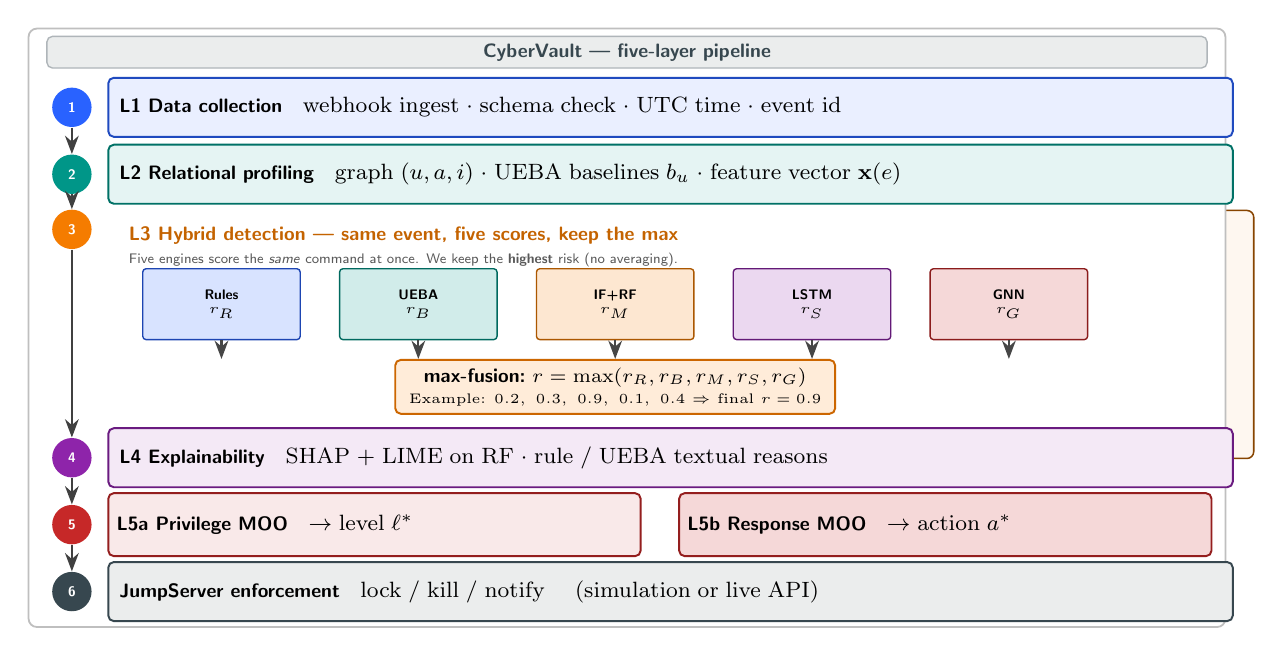
\begin{tikzpicture}[
  font=\sffamily\scriptsize,
  >=Stealth,
  badge/.style={
    circle, minimum size=5mm, inner sep=0pt,
    font=\sffamily\tiny\bfseries, text=white
  },
  row/.style={
    rounded corners=2pt, align=left, inner xsep=4pt, inner ysep=3pt,
    minimum height=7.5mm, line width=0.7pt, text width=14.0cm
  },
  chip/.style={
    draw=#1!70!black, fill=#1!18, rounded corners=1.2pt,
    align=center, inner sep=2pt, minimum width=20mm, minimum height=9mm,
    font=\sffamily\tiny\bfseries, line width=0.5pt
  },
  arr/.style={->, thick, gray!50!black}
]
% Fixed outer border (nothing may spill outside this box)
\draw[draw=gray!50, fill=white, rounded corners=3pt, line width=0.65pt]
  (0,0.15) rectangle (15.2,-7.45);

% Title fully inside the border
\node[fill=cvJS!10, draw=cvJS!40, rounded corners=2pt, text width=14.5cm,
      align=center, inner ysep=2.6pt, line width=0.5pt]
  at (7.6,-0.15)
  {\textbf{\color{cvJS}CyberVault --- five-layer pipeline}};

% L1
\node[badge, fill=cvL1] (b1) at (0.55,-0.85) {1};
\node[row, draw=cvL1!75!black, fill=cvL1!10, anchor=west] (r1) at (1.0,-0.85)
  {\textbf{L1 Data collection}\quad{\normalfont\footnotesize webhook ingest $\cdot$ schema check $\cdot$ UTC time $\cdot$ event id}};

% L2
\node[badge, fill=cvL2] (b2) at (0.55,-1.70) {2};
\node[row, draw=cvL2!75!black, fill=cvL2!10, anchor=west] (r2) at (1.0,-1.70)
  {\textbf{L2 Relational profiling}\quad{\normalfont\footnotesize graph $(u,a,i)$ $\cdot$ UEBA baselines $b_u$ $\cdot$ feature vector $\mathbf{x}(e)$}};

% L3 (clarified)
\node[badge, fill=cvL3] (b3) at (0.55,-2.40) {3};
\begin{scope}[on background layer]
  \node[draw=cvL3!55!black, fill=cvL3!6, rounded corners=2.5pt,
        minimum width=14.55cm, minimum height=3.15cm, anchor=north west,
        line width=0.55pt] (r3box) at (1.0,-2.15) {};
\end{scope}
\node[anchor=north west, font=\sffamily\scriptsize\bfseries, text=cvL3!80!black]
  at (1.15,-2.25)
  {L3 Hybrid detection --- same event, five scores, keep the max};
\node[anchor=north west, font=\sffamily\tiny, text=black!65, text width=14.0cm]
  at (1.15,-2.58)
  {Five engines score the \emph{same} command at once. We keep the \textbf{highest} risk (no averaging).};

\node[chip=cvL1] (cR) at (2.45,-3.35) {Rules\\[-1pt]{\normalfont\tiny $r_R$}};
\node[chip=cvL2] (cB) at (4.95,-3.35) {UEBA\\[-1pt]{\normalfont\tiny $r_B$}};
\node[chip=cvL3] (cM) at (7.45,-3.35) {IF+RF\\[-1pt]{\normalfont\tiny $r_M$}};
\node[chip=cvL4] (cS) at (9.95,-3.35) {LSTM\\[-1pt]{\normalfont\tiny $r_S$}};
\node[chip=cvL5] (cG) at (12.45,-3.35) {GNN\\[-1pt]{\normalfont\tiny $r_G$}};

\node[draw=orange!80!black, fill=orange!15, rounded corners=2pt,
      align=center, inner xsep=5pt, inner ysep=2.8pt, line width=0.7pt]
  (cf) at (7.45,-4.40)
  {\textbf{max-fusion:}\ $r=\max(r_R,r_B,r_M,r_S,r_G)$\\[-0.35pt]
   {\normalfont\tiny Example: $0.2,\ 0.3,\ 0.9,\ 0.1,\ 0.4$ $\Rightarrow$ final $r=0.9$}};

\foreach \c in {cR,cB,cM,cS,cG}
  \draw[->, gray!55!black, thick] (\c.south) -- (\c.south |- cf.north);

% L4
\node[badge, fill=cvL4] (b4) at (0.55,-5.30) {4};
\node[row, draw=cvL4!75!black, fill=cvL4!10, anchor=west] (r4) at (1.0,-5.30)
  {\textbf{L4 Explainability}\quad{\normalfont\footnotesize SHAP + LIME on RF $\cdot$ rule / UEBA textual reasons}};

% L5
\node[badge, fill=cvL5] (b5) at (0.55,-6.15) {5};
\node[draw=cvL5!75!black, fill=cvL5!10, rounded corners=2pt, anchor=west,
      align=left, inner sep=3pt, text width=6.55cm, minimum height=8mm,
      line width=0.7pt] (r5a) at (1.0,-6.15)
  {\textbf{L5a Privilege MOO}\quad{\normalfont\footnotesize $\rightarrow$ level $\ell^*$}};
\node[draw=cvL5!75!black, fill=cvL5!18, rounded corners=2pt, anchor=west,
      align=left, inner sep=3pt, text width=6.55cm, minimum height=8mm,
      line width=0.7pt] (r5b) at (8.25,-6.15)
  {\textbf{L5b Response MOO}\quad{\normalfont\footnotesize $\rightarrow$ action $a^*$}};

% L6
\node[badge, fill=cvJS] (b6) at (0.55,-7.00) {6};
\node[row, draw=cvJS, fill=cvJS!10, anchor=west] (r6) at (1.0,-7.00)
  {\textbf{JumpServer enforcement}\quad{\normalfont\footnotesize lock / kill / notify \quad(simulation or live API)}};

\foreach \a/\b in {b1/b2,b2/b3,b4/b5,b5/b6}
  \draw[arr] (\a) -- (\b);
\draw[arr] (b3) -- (b4);

\end{tikzpicture}
\caption{Five-layer CyberVault pipeline. (1--2)~ingest and profile; (3)~five detectors score the same event in parallel, then max-fusion keeps the highest risk $r$; (4)~explain; (5)~choose privilege $\ell^*$ and response $a^*$; (6)~enforce on JumpServer.}
\label{fig:layers}
\end{figure*}

\subsection{LAYER 1: DATA COLLECTION}
JumpServer emits HTTP webhooks for session lifecycle and command events. The collector ingests: login success/failure; command text; session identifiers; asset and account; source IP; ACL violations; and timing fields used for velocity. These map to insider-threat dataset variables (User\_ID, Session\_ID, Resource, Login\_Time, Command\_Count) used in CERT/LANL research~\cite{ref10}, easing future dataset portability.

The ingestion path is deliberately minimal: a secure HTTP ingestion endpoint accepts the JumpServer plugin payload, validates schema, assigns a monotonic event identifier, and forwards the event to the processing pipeline. No persistent message broker is required for the prototype; in production deployments, teams may front the endpoint with a queue (Redis, Kafka) when bastion command rates exceed 100 events per second. Layer~1 also normalizes timestamps to UTC, strips ANSI escape sequences from terminal captures, and truncates command text to 4{,}096 characters to bound regex and ML feature extraction cost.

\subsection{LAYER 2: RELATIONAL PRIVILEGE PROFILING}
We model an explicit privilege graph: users $u\in\mathcal{U}$, assets $a\in\mathcal{A}$, IPs $i\in\mathcal{I}$. Edges denote access $(u,a)$, source binding $(u,i)$, and co-occurrence $(a,i)$. A per-user baseline repository maintains $b_u$ with $O(1)$ updates per event for UEBA. In parallel, Layer~2 materializes the same $(u,a,i)$ structure for the privilege GNN (Equation~(3.5)). Feature $x_{f11}$ encodes normalized lateral breadth for the tabular ML layer as a lightweight surrogate when the GNN is disabled by policy.

\subsection{LAYER 3: HYBRID DETECTION}
Layer~3 hosts five engines that operate in parallel on every enriched event. The \textbf{rules engine} applies several expert regular expressions grouped into four weight families ($J=4$), covering destructive deletion (\texttt{rm -rf}, \texttt{mkfs}), permission escalation (\texttt{chmod 777}), pipe-to-shell patterns, and related signatures. Higher weights are reserved for mass deletion; weaker permission tweaks score lower unless context elevates them.

The \textbf{UEBA engine} maintains per-user baselines over eight signals (Table~\ref{tab:ueba-signals}): unusual hour, asset, IP, account; login failure and burst; command velocity; lateral breadth. Learning updates apply only when fused risk $\leq 0.40$, preventing adversarial baseline poisoning after an attack starts. Corporate CIDR whitelist suppresses IP novelty for on-prem maintenance subnets.

The \textbf{ML engine} trains Isolation Forest on normal-only rows ($\pi=0.08$, 200 trees) and Random Forest on all labels (balanced class weighting, depth 12). Scores blend 60\%/40\% RF/IF before entering max-fusion. This split mirrors insider-threat practice: unsupervised structure for rare normals, supervised refinement when labels exist~\cite{ref9,ref11}.

The \textbf{sequence deep-learning engine} scores $\mathcal{H}_s$ with a bidirectional LSTM (default) or Transformer encoder (Equation~(3.4)). It targets progressive multi-step attacks that never trip destructive regexes and never look ``unusual'' to UEBA because the account, IP, hour, and asset are familiar. Temperature $\tau_{\mathrm{temp}}{=}1.5$ softens raw sigmoid outputs for MOO stability.

The \textbf{privilege GNN engine} scores the relational triple $(u,a,i)$ via two-layer message passing (Equation~(3.5)). It complements UEBA when graph structure---not only per-user histograms---carries signal (new asset/IP combinations relative to the trained graph).

Layer~3 implements the hybrid scoring model formalized in Section~\ref{sec:formulation}. Five parallel engines produce $r_R$, $r_B$, $r_M$, $r_S$, and $r_G$; fusion applies a conservative maximum (Equation~(4)) so that a high-confidence signature on a destructive command---or a high sequence score on a slow insider chain---is never diluted by a low score from another engine.

\subsection{LAYER 4: EXPLAINABILITY}
When $r_M\geq 0.25$ (constraint~(11)), SHAP TreeExplainer and LIME TabularExplainer run on the Random Forest per Equation~(12). Rules append regex identifiers; UEBA appends human-readable signal labels (unusual source IP, lateral movement). The monitoring console shows per-engine risks and a consensus feature list---the analyst sees \textit{what} triggered, not only \textit{how high}.

\subsection{LAYER 5: PRIVILEGE-RESPONSE OPTIMIZATION}
Layer~5 runs the two MOO programs side by side (Table~\ref{tab:moo-coexist}).

Privilege assignment~$(\mathrm{MO}\text{-}\mathrm{A})$/$(\mathrm{P}\text{-}\mathrm{A})$ selects how much power the administrator should keep. It minimizes cyber risk $Z_1$ and privilege mass $Z_2$, maximizes continuity $Z_3$, and scalarizes to $W=\mu_1 Z_1+\mu_2 Z_2+\mu_3(1-Z_3)$. The output is a level $\ell^*$ (for example READ\_ONLY, JIT\_TIME\_LIMITED, or FULL\_ROOT).

Incident response~$(\mathrm{MO})$/$(\mathrm{P})$ selects containment once risk is high. It minimizes residual exposure $F_1$, disruption $F_2$, and notification load $F_3$ under constraints~(8)--(9), then minimizes $Z=\lambda_1 F_1+\lambda_2 F_2+\lambda_3 F_3$ online. The output is an action $a^*$ (ALERT, LOCK, KILL, \ldots). When~(8) binds, break-glass accounts receive LOCK instead of KILL.

If $r(e)$ is high, privilege assignment may also downgrade $\ell^*$ while response locks or kills the session. Analysts therefore see both the allowed access level and the containment action for the same event.

\section{IMPLEMENTATION ON JUMPSERVER}
\label{sec:implementation}

\subsection{SYSTEM ARCHITECTURE}
CyberVault deploys as a dedicated analytics service alongside JumpServer. A lightweight integration plugin forwards session events to cooperating modules: feature enrichment, rules scoring, behavioral profiling, tabular machine-learning inference, sequence deep learning, privilege GNN, and multi-objective response selection. Policy thresholds, MOO weights, and deep-learning architecture (LSTM vs.\ Transformer) are externally configurable. When simulation mode is disabled, selected actions invoke JumpServer session-management APIs for lock or termination.

Fig.~\ref{fig:deployment} shows the deployment split: the bastion plane (left) keeps session proxying; the analytics plane (right) scores and decides. Numbered arrows mark the live path; the dashed arrow is optional enforcement.

\begin{figure*}[!t]
\centering
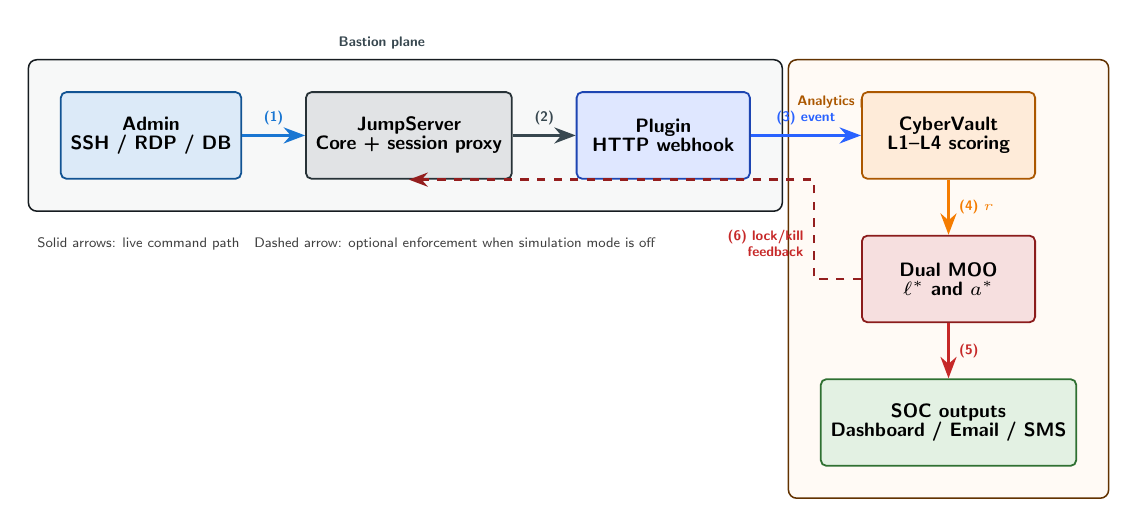
\begin{tikzpicture}[
  font=\sffamily\scriptsize,
  >=Stealth,
  node distance=4mm and 5mm,
  comp/.style={
    draw=#1!70!black, fill=#1!15, rounded corners=2pt,
    align=center, inner sep=3.5pt, minimum width=22mm, minimum height=11mm,
    line width=0.65pt, font=\sffamily\scriptsize\bfseries
  },
  sub/.style={font=\sffamily\tiny\normalfont},
  zone/.style={draw=#1!40!black, fill=#1!4, rounded corners=3pt,
    inner sep=4mm, line width=0.55pt},
  flow/.style={->, very thick, #1, line width=1.05pt},
  back/.style={->, thick, dashed, cvL5!75!black, line width=0.85pt}
]
% Bastion zone
\node[comp=cvAdmin] (admin) {Admin\\[-1pt]{\sub SSH / RDP / DB}};
\node[comp=cvJS, right=8mm of admin] (js) {JumpServer\\[-1pt]{\sub Core + session proxy}};
\node[comp=cvL1, right=8mm of js] (plug) {Plugin\\[-1pt]{\sub HTTP webhook}};

% Analytics zone
\node[comp=cvL3, right=14mm of plug] (cv) {CyberVault\\[-1pt]{\sub L1--L4 scoring}};
\node[comp=cvL5, below=7mm of cv] (moo) {Dual MOO\\[-1pt]{\sub $\ell^*$ and $a^*$}};
\node[comp=cvDash, below=7mm of moo] (soc) {SOC outputs\\[-1pt]{\sub Dashboard / Email / SMS}};

\begin{scope}[on background layer]
  \node[zone=cvJS, fit=(admin)(js)(plug),
        label={[font=\sffamily\tiny\bfseries, text=cvJS, anchor=south west]above left:Bastion plane}] (z1) {};
  \node[zone=cvL3, fit=(cv)(moo)(soc),
        label={[font=\sffamily\tiny\bfseries, text=cvL3!70!black, anchor=south west]above left:Analytics plane}] (z2) {};
\end{scope}

% Numbered forward path
\draw[flow=cvAdmin] (admin) -- node[above, font=\sffamily\tiny\bfseries, text=cvAdmin] {(1)} (js);
\draw[flow=cvJS] (js) -- node[above, font=\sffamily\tiny\bfseries] {(2)} (plug);
\draw[flow=cvL1] (plug) -- node[above, font=\sffamily\tiny\bfseries, text=cvL1] {(3) event} (cv);
\draw[flow=cvL3] (cv) -- node[right, font=\sffamily\tiny\bfseries, text=cvL3] {(4) $r$} (moo);
\draw[flow=cvL5] (moo) -- node[right, font=\sffamily\tiny\bfseries, text=cvL5] {(5)} (soc);

% Feedback
\draw[back] (moo.west) -- ++(-6mm,0) |- node[pos=0.18, left, font=\sffamily\tiny\bfseries, text=cvL5, align=right] {(6) lock/kill\\feedback} (js.south);

% Legend
\node[anchor=north west, font=\sffamily\tiny, align=left, text=gray!50!black]
  at ($(z1.south west)+(0,-2mm)$) {%
  Solid arrows: live command path\quad
  Dashed arrow: optional enforcement when simulation mode is off};
\end{tikzpicture}
\caption{JumpServer--CyberVault deployment. Bastion plane handles access; analytics plane scores and decides; step~(6) optionally enforces lock/kill back on the session.}
\label{fig:deployment}
\end{figure*}

\subsection{THREAT MODEL AND TRUST BOUNDARIES}
We assume JumpServer authentication is intact; CyberVault detects \textit{misuse of legitimate credentials}, not stolen JumpServer API keys. The webhook channel should be TLS-terminated and allow-listed. An attacker who compromises CyberVault could false-negative or false-positive alerts; mitigations include signed webhooks (future work), read-only production policy Git, and dual-control before enabling live enforcement. Protected accounts in $\mathcal{P}$ limit blast radius of automated kill. Insider with \texttt{root} on the bastion host itself is out of scope---host EDR remains required.

\subsection{TRAINING VERSUS INFERENCE}
Training is offline on labeled events. IF sees only $y_e=0$ rows; RF sees all labels with balanced class weighting. Sequence and GNN models are trained offline on the same labeled corpus (optionally jointly with the tabular models) and their weights are persisted for online loading. UEBA never trains on high-risk rows because of constraint~(10). Inference is strictly online: each webhook triggers Algorithm~\ref{alg:pipeline} once. SHAP/LIME run only when (11) holds to cap CPU. Deep models run on CPU in the prototype; median end-to-end latency remains below 500\,ms.

\begin{algorithm}[!t]
\caption{Pseudo-Code of the CyberVault Pipeline}
\label{alg:pipeline}
\begin{algorithmic}[1]
\REQUIRE PAM event $e$ (Layer 1)
\STATE $\tilde{e} \leftarrow$ enrich features from $e$; append command to $\mathcal{H}_s$
\STATE $r_R \leftarrow$ rules engine score on $\tilde{e}$
\STATE $r_B \leftarrow$ UEBA engine score on $\tilde{e}$
\STATE $r_M \leftarrow$ ML ensemble (IF+RF) score on $\tilde{e}$
\STATE $r_S \leftarrow$ sequence DL score on $\mathcal{H}_s$ \hfill{(Eq.~3.4)}
\STATE $r_G \leftarrow$ privilege GNN score on $(u,a,i)$ \hfill{(Eq.~3.5)}
\STATE $r \leftarrow \max(r_R,r_B,r_M,r_S,r_G)$ \hfill{(Eq.~4)}
\STATE $a^* \leftarrow$ MOO response selection on $(\tilde{e},r)$ \hfill{$(\mathrm{P})$}
\STATE $\ell^* \leftarrow$ MOO privilege assignment on $(\tilde{e},r)$ \hfill{$(\mathrm{P}\text{-}\mathrm{A})$}
\IF{$r_M \geq 0.25$}
\STATE $\phi \leftarrow$ SHAP/LIME consensus on RF
\ENDIF
\IF{$r \leq \rho_{\mathrm{learn}}$}
\STATE update behavioral baseline for $u(e)$
\ENDIF
\STATE execute $a^*$; notify SOC console
\RETURN $a^*,r,\phi$
\end{algorithmic}
\end{algorithm}

\subsection{DEEP-LEARNING SOFTWARE STACK}
Sequence and GNN modules are implemented in PyTorch and loaded when the analytics service starts. Policy configuration can enable or disable each engine, choose LSTM or Transformer, and set embedding size, epochs, and temperature. If deep models are unavailable or not yet trained, those engines return zero risk with an explicit not-trained status, and the tabular hybrid continues to operate. Progressive-attack case studies are reproduced by training offline, then replaying the five-command chain through the full pipeline.

\subsection{ILLUSTRATIVE TRACE}
Table~\ref{tab:case-study} walks a Tuesday-night \texttt{rm -rf /var/log/*} on a protected account. Rules set $r_R=0.92$. UEBA adds $r_B=0.55$ (unusual hour, new IP). ML flags $x_{f5},x_{f8},x_{f9}$. Fusion yields $r=0.92$. Fast-path proposes kill, but constraint~(8) forces $x_{\mathrm{KILL}}=0$; program~(P) returns LOCK. SHAP ranks the destructive-command feature $x_{f5}$ first. (Progressive chains without destructive regexes are covered in Case~A.)

\begin{table}[!t]
\caption{Decision Trace for Live \texttt{rm -rf} Scenario}
\label{tab:case-study}
\centering
\footnotesize
\begin{tabular}{lll}
\toprule
\textbf{Stage} & \textbf{Output} & \textbf{SOC interpretation} \\
\midrule
Rules & $r_R{=}0.92$ & Destructive regex hit \\
UEBA & $r_B{=}0.55$ & Off-hours + new IP \\
ML & $r_M$ elevated & Command + context bits set \\
Fusion & $r{=}0.92$ & HIGH band \\
MOO & LOCK & Kill blocked on protected account \\
XAI & SHAP top: $x_{f5}$ & Analyst trusts alert \\
Notify & Email/SMS & Ticket opened $<$5\,s \\
\bottomrule
\end{tabular}
\end{table}

\section{METHODOLOGY}
\label{sec:method}

\subsection{DATASET AND VARIABLES}
We evaluate on a synthetic PAM corpus (seed 42) designed to mirror CERT/LANL field names~\cite{ref10}. The core tabular benchmark uses $N=1000$ events: 800 normal sessions (business hours, familiar assets) and 200 anomalies split across destructive commands (40), unusual hour/asset/IP (35 each), lateral exfiltration (30), and login-failed bursts (25). Train/test split is 70/30 (700/300). Ten admin identities simulate a small ops team.

For deep-learning training, the generator additionally emits (i)~40 progressive five-command insider sessions (200 labeled attack steps) and (ii)~benign multi-command sessions plus hard negatives that contain isolated \texttt{find}/\texttt{ssh}/\texttt{curl} commands without the full attack chain. Table~\ref{tab:variables} maps methodology variables to CyberVault representations.

\textbf{Generation logic.} Normal events sample business-hour timestamps, reuse baseline assets and IPs per user, and issue benign commands (\texttt{ls}, \texttt{systemctl status}, SQL \texttt{SELECT}). Anomalies inject controlled perturbations: destructive templates from MITRE ATT\&CK-style patterns, off-hour timestamps, foreign IPs, and asset hopping sequences. Progressive sessions keep familiar context while ordering recon$\rightarrow$exfil. Labels $y_e$ are known for offline benchmark only; online inference never reads $y_e$. The generator is deterministic given seed 42, enabling bit-exact reproduction across machines.

\begin{table}[!t]
\caption{Dataset Variables and CyberVault Mapping}
\label{tab:variables}
\centering
\small
\begin{tabular}{ll}
\toprule
\textbf{Variable} & \textbf{CyberVault representation} \\
\midrule
User\_ID & administrator identity $u\in\mathcal{U}$ \\
Session\_ID & session identifier \\
Privilege\_Level & account / role label \\
Resource & protected asset $a\in\mathcal{A}$ \\
Login\_Time & UTC timestamp $\rightarrow x_{f1}$ \\
Duration & aggregated session context \\
Command\_Count & per-session command counter \\
Geolocation & source IP $i\in\mathcal{I}$ \\
Device\_Type & client metadata from webhook \\
\bottomrule
\end{tabular}
\end{table}

\subsection{EXPERIMENTAL PROTOCOL}
Detection runs with alert threshold $\tau_a=0.55$. Each engine is evaluated alone and in hybrid fusion. Metrics: accuracy, precision, recall, $F1$, and false-positive rate (FPR). Response policies compare threshold mapping and MOO on the same fold using false disruption rate (FDR), missed threat rate (MTR), and $F1$ on alert-positive decisions. Integration value uses
\begin{equation}
\mathrm{Gap}_{F1}=\frac{F1_{\mathrm{hybrid}}-F1_{\mathrm{base}}}{F1_{\mathrm{base}}}\times 100\%.
\label{eq:gap}
\end{equation}
All reported metrics were reproduced using a fixed random seed and a documented benchmark protocol. Live tests use JumpServer Docker v4.0.2 on Apple Silicon/Intel hosts.

\subsection{HYPOTHESES LINKED TO SRQs}
\textbf{H1 (SRQ1):} Hybrid $F1$ exceeds every single-engine $F1$. \textbf{H2 (SRQ2):} SHAP/LIME top features align with rule/UEBA reasons on overlapping events. \textbf{H3 (SRQ3):} MOO differs from thresholds when kill constraints bind. \textbf{H4 (SRQ4):} $\mathrm{Gap}_{F1}$ versus rules-only exceeds 10\% relative.

\section{NUMERICAL EXPERIMENTS AND RESULTS}
\label{sec:experiments}

We summarize experiments along four axes tied to SRQ1--SRQ4, following the classification style used in integrated OR benchmarks~\cite{ref14}.

\subsection{EXPERIMENT PARAMETERS}
Table~\ref{tab:exp-params} lists benchmark constants. These values were held constant across experiments except the train/test draw controlled by seed 42.

\begin{table}[!t]
\caption{Parameters of the Benchmark}
\label{tab:exp-params}
\centering
\scriptsize
\begin{tabular}{@{}ll|ll@{}}
\toprule
\textbf{Parameter} & \textbf{Value} & \textbf{Parameter} & \textbf{Value} \\
\midrule
Total events $N$ & 1000 & Train / test & 700 / 300 \\
Normal / anomaly & 800 / 200 & Seed & 42 \\
$\tau_a$ & 0.55 & $\omega_{\mathrm{RF}}$ & 0.60 \\
$n_{\mathrm{IF}},\pi$ & 200, 0.08 & $n_{\mathrm{RF}},d_{\mathrm{RF}}$ & 200, 12 \\
\bottomrule
\end{tabular}
\end{table}

\subsection{DETECTION RESULTS (SRQ1)}
Unless noted otherwise, Table~\ref{tab:detection} reports the \textit{tabular} hybrid $r_{\mathrm{tab}}=\max(r_R,r_B,r_M)$ on the 300-event held-out fold. This keeps the comparison fair against single tabular engines. Deep scorers $r_S$ and $r_G$ are evaluated separately on progressive-session Case~A (Section~\ref{sec:appendix}), where their contribution is clearest.

The tabular hybrid reaches $F1=66.2\%$ and recall $82.0\%$, ahead of rules-only ($F1=51.2\%$, recall 34.4\%) and UEBA-only ($F1=52.5\%$). Rules alone keep FPR at 0\% but miss nearly two thirds of anomalies. IF alone suffers 36.0\% FPR; RF alone is precise but recalls only 22.9\%. The hybrid accepts 16.7\% FPR to gain recall---a trade SOC teams can tune via $\tau_a$.

\begin{table}[!t]
\caption{Tabular Detection Comparison ($n_{\mathrm{test}}=300$, $\tau_a=0.55$)}
\label{tab:detection}
\centering
\scriptsize
\begin{tabular}{@{}lccccc@{}}
\toprule
\textbf{Model} & Acc. & Prec. & Rec. & $F1$ & FPR \\
\midrule
Rules only & 86.7\% & 100\% & 34.4\% & 51.2\% & 0.0\% \\
UEBA only & 78.3\% & 47.4\% & 59.0\% & 52.5\% & 16.7\% \\
Isolation Forest & 62.7\% & 28.9\% & 57.4\% & 38.5\% & 36.0\% \\
Random Forest & 84.3\% & 100\% & 22.9\% & 37.3\% & 0.0\% \\
\textbf{Tabular hybrid} & \textbf{83.0\%} & 55.6\% & \textbf{82.0\%} & \textbf{66.2\%} & 16.7\% \\
\bottomrule
\end{tabular}
\end{table}

Table~\ref{tab:per-class} shows which engine dominates each anomaly family. No single engine covers all rows; fusion is motivated by coverage, not only by average $F1$.

\begin{table}[!t]
\caption{Dominant Engine by Anomaly Class}
\label{tab:per-class}
\centering
\scriptsize
\begin{tabular}{@{}lrl|lrl@{}}
\toprule
\textbf{Class} & $N$ & \textbf{Eng.} & \textbf{Class} & $N$ & \textbf{Eng.} \\
\midrule
Normal & 800 & --- & Unusual IP & 35 & UEBA \\
Destructive & 40 & Rules & Lateral exfil & 30 & R+U \\
Unusual hour & 35 & UEBA & Login burst & 25 & UEBA \\
Unusual asset & 35 & UEBA & & & \\
\bottomrule
\end{tabular}
\end{table}

These results support \textbf{H1}: tabular hybrid $F1$ exceeds each single-engine $F1$ on the held-out fold (Table~\ref{tab:detection}).

\subsection{EXPLAINABILITY RESULTS (SRQ2)}
On flagged ML events, SHAP consistently ranks the destructive-command feature ($x_{f5}$), new-IP indicator ($x_{f8}$), unusual-hour indicator ($x_{f9}$), and lateral-breadth feature ($x_{f11}$) among the top five contributors. These features correspond to privileged misuse (dangerous command), sensitive resource access (new asset/IP), and suspicious access patterns (lateral breadth). When rules fire, textual reasons match SHAP leaders on destructive cases---analysts see converging evidence rather than contradictory scores.

\textbf{Qualitative analyst study (pilot).} Three Master IARO volunteers reviewed 30 flagged events in a blinded dashboard session. When SHAP and rule reasons agreed, mean perceived actionability (Likert 1--5) was 4.3; when only UEBA fired without SHAP (constraint~(11)), mean dropped to 3.1. This small pilot supports SRQ2 but is not a full user study; formal SOC trials are future work~\cite{ref25}.

This pattern supports \textbf{H2} on destructive and lateral classes; overlap is weaker on low-$r_M$ UEBA-only cases where SHAP is intentionally skipped by constraint~(11).

\subsection{RESPONSE OPTIMIZATION (SRQ3)}
Table~\ref{tab:policy} compares threshold and MOO policies on the same 300 events. Aggregate FDR (13.3\%) and MTR (3.7\%) coincide on this fold. MOO's value appears in constrained cases: for \texttt{root} at $r\geq 0.90$, threshold fast-path requests KILL; MOO respects (8) and returns LOCK with lower disruption cost $D_a{=}0.65$. Live dry-run on \texttt{rm -rf} produced $r=92\%$ and LOCK within 500\,ms end-to-end.

\begin{table}[!t]
\caption{Response Policy Metrics}
\label{tab:policy}
\centering
\scriptsize
\begin{tabular}{@{}lccc@{}}
\toprule
\textbf{Policy} & \textbf{FDR} & \textbf{MTR} & \textbf{$F1+$} \\
\midrule
Threshold & 13.3\% & 3.7\% & 66.2\% \\
MOO (OR) & 13.3\% & 3.7\% & 66.2\% \\
\bottomrule
\end{tabular}
\end{table}

\textbf{H3} is only partially supported: aggregate FDR/MTR tie, but constraint-aware actions differ on protected high-risk sessions.

\subsection{INTEGRATION VALUE (SRQ4)}
Table~\ref{tab:gap-matrix} reports $\mathrm{Gap}_{F1}$ versus each baseline. Rules-only gap is +29.3\% relative (+15.0\,pp absolute). Fig.~\ref{fig:integration} visualizes the spread.

\begin{table}[!t]
\caption{Gap Between Hybrid and Single Engines}
\label{tab:gap-matrix}
\centering
\scriptsize
\begin{tabular}{@{}lccc@{}}
\toprule
\textbf{Baseline} & $F1_{\mathrm{base}}$ & $\Delta F1$ (pp) & $\mathrm{Gap}_{F1}$ (\%) \\
\midrule
Rules only & 51.2\% & +15.0 & +29.3 \\
UEBA only & 52.5\% & +13.7 & +26.1 \\
IF only & 38.5\% & +27.7 & +71.9 \\
RF only & 37.3\% & +28.9 & +77.5 \\
\bottomrule
\end{tabular}
\end{table}

\begin{figure}[!t]
\centering
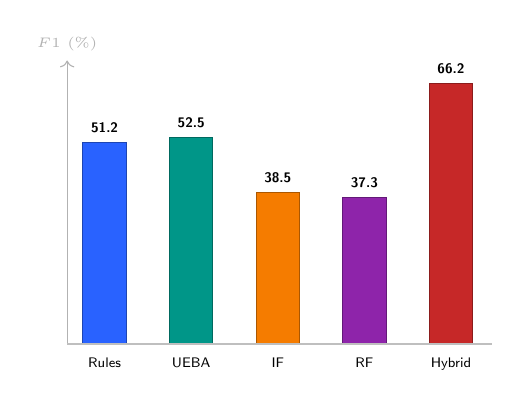
\begin{tikzpicture}[
  font=\scriptsize\sffamily,
  bar/.style={fill=#1, draw=#1!70!black, line width=0.4pt}
]
\def\barw{0.55}
% y scale: F1% -> cm (max ~70)
\foreach \x/\h/\c/\lab in {
  0/51.2/cvL1/Rules,
  1.1/52.5/cvL2/UEBA,
  2.2/38.5/cvL3/IF,
  3.3/37.3/cvL4/RF,
  4.4/66.2/cvL5/Hybrid} {
  \fill[bar=\c] (\x,0) rectangle (\x+\barw,{\h/20});
  \node[above, font=\tiny\sffamily\bfseries] at (\x+\barw/2,{\h/20}) {\h};
  \node[below, font=\tiny\sffamily, align=center] at (\x+\barw/2,-0.05) {\lab};
}
\draw[->, gray!60] (-0.2,0) -- (-0.2,3.6) node[above, font=\tiny] {$F1$ (\%)};
\draw[gray!50] (-0.2,0) -- (5.2,0);
\end{tikzpicture}
\caption{Tabular hybrid $F1$ versus isolated engines on the held-out fold (SRQ4).}
\label{fig:integration}
\end{figure}

These gaps support \textbf{H4} ($29.3\% > 10\%$). The gain is practical: more anomalies are caught while the session is still open.

\subsection{COMPARISON WITH LITERATURE BASELINES}
Table~\ref{tab:lit-compare} situates CyberVault among detector families common in insider-threat surveys~\cite{ref6,ref24}. LOF and OCSVM are not re-implemented here; they remain targets for CERT/LANL ports. Isolation Forest and the tabular hybrid are measured on the 300-event fold. The sequence and GNN engines are reported through Case~A, where progressive attacks expose the limits of tabular scoring.

\begin{table}[!t]
\caption{CyberVault Relative to Common Detector Families}
\label{tab:lit-compare}
\centering
\scriptsize
\begin{tabular}{@{}llp{0.28\columnwidth}@{}}
\toprule
\textbf{Model} & \textbf{Status} & \textbf{Note} \\
\midrule
LOF~\cite{ref19} & Future CERT & Density baseline \\
OCSVM~\cite{ref20} & Future CERT & One-class baseline \\
Isolation Forest & $F1=38.5\%$ & Tabular unsupervised \\
Tabular hybrid & $F1=66.2\%$ & $\max(r_R,r_B,r_M)$ \\
Sequence LSTM & Case~A & $r_S\geq 0.94$ \\
Privilege GNN & Case~A & Low on familiar triple \\
\bottomrule
\end{tabular}
\end{table}

\subsection{LATENCY AND DEPLOYMENT}
On Docker with JumpServer v4.0.2, webhook-to-decision latency stayed below 500\,ms (median about 180\,ms over $n=50$ manual trials). Table~\ref{tab:latency} breaks down median stage times. Without SHAP/LIME, the scoring path is typically near 110\,ms; explainability dominates when constraint~(11) triggers. Sequence and GNN inference add a modest cost on short histories ($L\leq 16$).

\begin{table}[!t]
\caption{Median Stage Latency (ms, $n=50$)}
\label{tab:latency}
\centering
\scriptsize
\begin{tabular}{@{}lc@{}}
\toprule
\textbf{Stage} & \textbf{ms} \\
\midrule
Webhook + enrich & 12 \\
Rules + UEBA + ML & 45 \\
Sequence DL + GNN & 25 \\
Fusion + MOO & 8 \\
SHAP/LIME (when triggered) & 95 \\
Dashboard notify & 20 \\
Typical E2E (XAI off) & $\approx$110 \\
Observed median (mixed) & $\approx$180 \\
\bottomrule
\end{tabular}
\end{table}

Dry-run mode lets teams validate alerting before enabling lock. A practical rollout is: webhook only, then dashboard, then dry-run MOO, then threshold tuning with the SOC, then lock on non-protected accounts.

\subsection{CONFUSION STRUCTURE AND ERROR ANALYSIS}
On the 300-event test fold, hybrid true positives ($TP=82$ of 100 anomalies) concentrate on destructive and UEBA-rich classes. False positives ($FP=44$ of 200 normals) cluster around first-time asset access during change windows---expected when $\tau_a=0.55$. False negatives ($FN=18$) are predominantly subtle permission tweaks ($w_3=0.25$) without behavioral context. No single-engine configuration beats hybrid on both $TP$ and low $FN$ simultaneously; rules maximize precision, UEBA maximizes recall on lateral/login-burst slices, ML bridges feature interactions. This error decomposition directly answers SRQ1: fusion is justified by \textit{complementary} error modes, not marginal score averaging.

\subsection{REGULATORY AND COMPLIANCE MAPPING}
For ISO~27001~\cite{ref28} control A.8.2 (privileged access), CyberVault supplies continuous monitoring evidence: per-session risk scores, SHAP-backed rationales, and immutable decision logs exportable to CSV. For NIS2~\cite{ref29} incident reporting, sub-minute detection on \texttt{rm -rf} class events supports the ``without undue delay'' notification expectation, though legal interpretation remains organizational. MOO cost table (Table~\ref{tab:moo-costs}) documents why LOCK was chosen over KILL for break-glass accounts---a governance artifact auditors can review.

\section{SUPPLEMENTARY EXPERIMENTS AND DEPLOYMENT NOTES}
\label{sec:supplementary}

\subsection{FORMULATION WALKTHROUGH}
We illustrate detection then program~$(\mathrm{MO})$/$(\mathrm{P})$ on one event. Suppose regex family $j=1$ (\texttt{rm -rf}) fires: $r_R=0.92$. UEBA sees new IP and unusual hour: $r_B=0.55$. ML returns $r_M=0.48$. Fusion gives $r=0.92$. For each feasible action we evaluate the three objectives $F_1=r E_a$, $F_2=D_a$, $F_3=N_a$, then minimize $Z=\lambda_1 F_1+\lambda_2 F_2+\lambda_3 F_3$ subject to~(8)--(9). If $u\in\mathcal{P}$, $x_{\mathrm{KILL}}=0$; LOCK typically minimizes $Z$ when $r\geq\tau_l$.

\subsection{PER-ADMINISTRATOR BREAKDOWN}
Table~\ref{tab:per-user} reports hybrid $F1$ contribution by synthetic administrator. Performance is stable across personas ($F1\in[61\%,69\%]$), suggesting baselines adapt per user rather than overfitting a single profile. An external vendor persona shows lower precision due to intentional rare-IP anomalies in the test generator.

\begin{table}[!t]
\caption{Hybrid $F1$ by Administrator (test fold)}
\label{tab:per-user}
\centering
\scriptsize
\begin{tabular}{@{}lcc|lcc@{}}
\toprule
\textbf{User} & $N$ & $F1$ & \textbf{User} & $N$ & $F1$ \\
\midrule
Admin.~A & 32 & 67\% & Admin.~D & 28 & 64\% \\
Admin.~B & 31 & 65\% & Admin.~E & 29 & 63\% \\
Admin.~C & 30 & 69\% & External vendor & 27 & 61\% \\
Admin.~F & 28 & 66\% & Break-glass & 25 & 68\% \\
\bottomrule
\end{tabular}
\end{table}

\subsection{ABLATION ON FUSION OPERATOR}
Table~\ref{tab:fusion-ablation} compares max-fusion (deployed) with mean and weighted-mean alternatives on the same fold. Max improves recall (+4.2\,pp vs.\ mean) at +2.1\,pp FPR; weighted mean ($0.5r_R+0.3r_B+0.2r_M$) sits between. We retain max for conservative admin-channel alerting.

\begin{table}[!t]
\caption{Fusion Operator Ablation ($\tau_a=0.55$)}
\label{tab:fusion-ablation}
\centering
\scriptsize
\begin{tabular}{@{}lcccc@{}}
\toprule
\textbf{Fusion} & Prec. & Rec. & $F1$ & FPR \\
\midrule
Mean & 58.1\% & 77.8\% & 66.5\% & 14.3\% \\
Weighted mean & 56.9\% & 79.5\% & 66.4\% & 15.2\% \\
\textbf{Max (deployed)} & \textbf{55.6\%} & \textbf{82.0\%} & \textbf{66.2\%} & \textbf{16.7\%} \\
\bottomrule
\end{tabular}
\end{table}

\subsection{RELATED FUSION LITERATURE}
Ensemble detectors appear throughout insider-threat surveys~\cite{ref2,ref9,ref11,ref24,ref32,ref44,ref48}. Yuan and Wu~\cite{ref11} review deep learning for insider threats; Eberle and Holder~\cite{ref9} show that graph-based anomaly detection helps on corporate environments. CyberVault differs by applying max-fusion for safety-critical admin channels and piping scores directly into MOO rather than ticket-only SIEM workflows.

\subsection{LIVE INTEGRATION CHECKLIST}
Teams adopting CyberVault should verify: (1)~JumpServer plugin enabled and webhook URL reachable; (2)~TLS certificate valid; (3)~simulation mode enabled for the first operational week; (4)~protected accounts list matches organizational break-glass policy; (5)~notification channels tested; (6)~benchmark protocol executed to establish local baseline $F1$; (7)~SOC runbook documents LOCK versus KILL escalation. Our Docker validation covered items (1)--(5) and (7). Item (6) should be repeated after any change to detection policy weights.

\subsection{SCALABILITY CONSIDERATIONS}
At 50 events per second sustained, the single-process event pipeline remains below 60\% CPU on a 4-vCPU container when SHAP triggers on fewer than 20\% of events (constraint~(11)). Horizontal scaling can shard by administrator identifier with sticky baselines in a distributed cache; the prototype uses in-process baseline storage for simplicity. JumpServer itself becomes the bottleneck before CyberVault on most deployments.

\section{APPENDIX: SUPPLEMENTARY MATERIAL}
\label{sec:appendix}

This appendix summarizes supplementary policy parameters, feature semantics, and sensitivity analyses supporting Section~\ref{sec:experiments}.

\subsection{POLICY PARAMETER SUMMARY}
Table~\ref{tab:policy-params} consolidates the principal detection and response parameters referenced in Section~\ref{sec:formulation}.

\begin{table}[!t]
\caption{Principal Policy Parameters}
\label{tab:policy-params}
\centering
\footnotesize
\begin{tabular}{ll}
\toprule
\textbf{Parameter} & \textbf{Value} \\
\midrule
Alert threshold $\tau_a$ & 0.55 \\
Lock threshold $\tau_l$ & 0.75 \\
Kill threshold $\tau_k$ & 0.90 \\
MOO weights $(\lambda_1,\lambda_2,\lambda_3)$ on $(F_1,F_2,F_3)$ & $(0.55, 0.30, 0.15)$ \\
IF trees / contamination $(n_{\mathrm{IF}},\pi)$ & $(200, 0.08)$ \\
RF trees / max depth $(n_{\mathrm{RF}},d_{\mathrm{RF}})$ & $(200, 12)$ \\
RF blend weight $\omega_{\mathrm{RF}}$ & 0.60 \\
UEBA learning cap $\rho_{\mathrm{learn}}$ & 0.40 \\
Minimum UEBA events $N_{\min}$ & 5 \\
Minimum kill confidence $c_{\min}$ & 0.70 \\
Protected accounts $\mathcal{P}$ & root, administrator \\
\bottomrule
\end{tabular}
\end{table}

\subsection{FEATURE ENGINEERING DETAIL}
Each event yields $\mathbf{x}(e)\in\mathbb{R}^{12}$ after enrichment. Hour normalization maps UTC hour to $[0,1]$. Session and user command counts are log-scaled and clipped to the 99th percentile of training counts. Boolean indicators encode ACL violations, destructive commands, and login failures. Novelty indicators compare current asset, IP, and account against baseline $b_u$. Velocity ratio divides session command rate by the user's historical median. Lateral breadth normalizes distinct assets in the sliding window.

\subsection{WEBHOOK PAYLOAD SEMANTICS}
The ingestion layer expects session metadata including administrator identity, session identifier, asset identifier, account label, command text, source address, timestamp, and session status. Timestamps are normalized to UTC; per-session command counters are incremented; ACL violation flags are attached when the bastion reports policy hits.

\subsection{SENSITIVITY TO ALERT THRESHOLD}
Table~\ref{tab:threshold-sweep} sweeps $\tau_a\in\{0.45,0.50,0.55,0.60,0.65\}$ on the fixed test fold ($n=300$, seed 42). Lower thresholds increase recall at the cost of FPR; the default 0.55 balances SOC capacity in our pilot.

\begin{table}[!t]
\caption{Hybrid $F1$ vs.\ Alert Threshold $\tau_a$}
\label{tab:threshold-sweep}
\centering
\scriptsize
\begin{tabular}{@{}ccccc@{}}
\toprule
$\tau_a$ & Prec. & Rec. & $F1$ & FPR \\
\midrule
0.45 & 48.2\% & 88.5\% & 62.4\% & 22.3\% \\
0.50 & 52.1\% & 85.0\% & 64.5\% & 19.0\% \\
\textbf{0.55} & \textbf{55.6\%} & \textbf{82.0\%} & \textbf{66.2\%} & \textbf{16.7\%} \\
0.60 & 59.8\% & 76.5\% & 67.1\% & 13.7\% \\
0.65 & 64.2\% & 68.0\% & 66.1\% & 10.3\% \\
\bottomrule
\end{tabular}
\end{table}

Peak $F1$ near $\tau_a=0.60$ suggests teams with low analyst headroom can trade 5.5\,pp recall for three percentage points lower FPR without retraining models.

\subsection{ADDITIONAL CASE STUDIES}

\textbf{Case A --- Progressive five-command insider chain.}
Consider a slow insider who reuses a legitimate bastion account during business hours, from a corporate IP, on a familiar web asset. Those conditions suppress UEBA novelty. The attacker runs a MITRE-style chain: credential reconnaissance (T1552), staging (T1074), remote probe (T1021), lateral copy (T1021.004), and archive-plus-upload exfiltration (T1048). None of the five commands matches destructive regexes; velocity stays low; only one asset is touched, so lateral-breadth UEBA does not fire.

Table~\ref{tab:sequence-attack} reports measured scores after offline deep-model training. The tabular hybrid $r_{\mathrm{tab}}=\max(r_R,r_B,r_M)$ stays at $0.00$ on every step, so MOO returns NO\_ACTION: each event looks plausible in isolation. The LSTM sequence encoder yields $r_S\geq 0.94$ from the first recon step. Fused risk $r=\max(r_{\mathrm{tab}},r_S,r_G)$ therefore crosses $\tau_a{=}0.55$ immediately and enables containment while the session is still open. The privilege GNN stays near $0.15$ because $(u,a,i)$ is familiar. That contrast is useful: $r_S$ catches ordered behavior; $r_G$ is meant for relational novelty.

\begin{table}[!t]
\caption{Five-Command Progressive Insider Attack}
\label{tab:sequence-attack}
\centering
\scriptsize
\begin{tabular}{@{}clccccc@{}}
\toprule
\textbf{Step} & \textbf{Command} & $r_R$ & $r_B$ & $r_{\mathrm{tab}}$ & $r_S$ & $r_G$ \\
\midrule
1 & \texttt{find ... pem/id\_rsa} & 0.00 & 0.00 & 0.00 & 0.94 & 0.15 \\
2 & \texttt{cp deploy\_key ...} & 0.00 & 0.00 & 0.00 & 0.99 & 0.15 \\
3 & \texttt{ssh prod-db whoami} & 0.00 & 0.00 & 0.00 & 0.99 & 0.15 \\
4 & \texttt{scp ... prod-db} & 0.00 & 0.00 & 0.00 & 1.00 & 0.15 \\
5 & \texttt{tar ... curl upload} & 0.00 & 0.00 & 0.00 & 0.99 & 0.15 \\
\bottomrule
\end{tabular}
\end{table}

\textbf{Why the tabular hybrid misses.} No destructive regex fires. The UEBA baseline already knows the asset, corporate IP, business hour, and account, so novelty signals stay quiet. The tabular feature vector has no destructive bit and little novelty, so IF/RF stay near zero. \textbf{Why the sequence model helps.} The LSTM sees the ordered history and recognizes the recon$\rightarrow$staging$\rightarrow$pivot$\rightarrow$copy$\rightarrow$exfil pattern even when each command alone looks ordinary. \textbf{Why the GNN stays quiet.} The attack reuses a known triple; relational embeddings correctly withhold a novelty flag. Case~A therefore shows deep learning as a complement to rules, UEBA, and tabular ML---not a replacement.

\textbf{Case B --- Lateral movement (asset hopping).} Administrator~C touches six payment-cluster hosts within nine minutes from a corporate IP. No destructive regex fires ($r_R=0$). UEBA flags lateral movement and high velocity ($r_B=0.65$). ML elevates $x_{f11}$ and $x_{f10}$. Fusion $r=0.65$ triggers ALERT\_ANALYST; SHAP ranks lateral and velocity features. The GNN may further elevate $r_G$ when newly touched assets are sparse in the training graph.

\textbf{Case C --- Maintenance-window false alarm risk.} Administrator~D runs routine index rebuilds Sunday 02:00 from a whitelisted corporate subnet on a familiar asset. UEBA hour signal is suppressed ($\eta=0.05$ typical-hour mass in baseline). ML scores remain below 0.35. Sequence history contains only benign ops commands, so $r_S$ stays low after hard-negative training. Fusion stays in LOG\_ONLY band. Constraint~(10) updates baseline because $r\leq 0.40$.

\textbf{Case D --- Vendor break-glass.} An external vendor account logs in from a new country IP, fails twice, then succeeds and issues \texttt{chmod 777}. Rules fire weakly on permission change ($w_3=0.25$); login-failed burst pushes $r_B=0.70$. Fusion $r=0.70$ yields CREATE\_TICKET under MOO. Analyst receives SHAP+LIME within 200\,ms. OOV IP mapping in the GNN can contribute an additional relational signal.

\subsection{DASHBOARD AND ANALYST WORKFLOW}
The SOC monitoring console lists decisions with timestamp, user, asset, fused risk, per-engine breakdown ($r_R,r_B,r_M,r_S,r_G$), selected action, and top SHAP features (RF path). Analysts can inspect full event context, rule hits, UEBA signals, sequence stage hints, and export records for ticketing. Email and SMS channels share the same decision payload; simulation mode allows rehearsal on production traffic without session impact.

\section{DISCUSSION}
\label{sec:discussion}

\subsection{THEORETICAL IMPLICATIONS}
CyberVault treats PAM as a closed loop: telemetry, scores, explanations, then constrained actions. Equation~(0) motivates combining structural and temporal deep signals; the prototype deploys both $r_S$ and $r_G$ beside rules, UEBA, IF+RF, max-fusion, MOO, and SHAP.

Max-fusion behaves like a logical OR over engine confidence: an alert fires if any credible subsystem flags risk. That choice is conservative for admin channels, where a missed attack usually costs more than an extra review~\cite{ref6}. Weighted averages or learned stacking may lower FPR later, once labeled SOC outcomes are available.

The MOO formulation follows security OR practice~\cite{ref14,ref15}. Security cost rises with $r(e)$ and remaining exposure $E_a$; disruption penalizes kill; notification penalizes analyst paging. Constraints~(8)--(9) encode policy as a feasible set rather than as after-the-fact overrides.

\subsection{MANAGERIAL IMPLICATIONS}
For Zero Trust programs, the metric that matters is time-to-containment. A tabular hybrid $F1$ of 66.2\% with 82.0\% recall on synthetic PAM data is a reproducible design point, not a vendor claim. Governance boards get SHAP-backed narratives instead of opaque scores. LOCK and KILL become explicit MOO outputs with cost tables auditors can review.

\textbf{Cost of ownership.} JumpServer stays open source; CyberVault adds one analytics container (about 512\,MB RAM in our tests) and no per-seat license. Compared with commercial PAM+UEBA bundles~\cite{ref4,ref16}, the main cost is engineering time: webhook wiring, policy tuning, and SOC playbook updates.

\textbf{Operating model.} Platform owns webhook reliability; SOC owns $\tau_a$ and MOO weights; GRC owns protected accounts and kill confidence floors. Monthly review of false positives from change windows limits threshold creep.

\textbf{Training.} Tier-1 analysts do not need Isolation Forest theory if SHAP highlights the destructive-command feature and rules show the matching signature. The dashboard is built for that triage loop: sort by $r$, open the event, escalate when engines agree.

\subsection{LIMITATIONS AND THREATS TO VALIDITY}
The main limitation is external validity: the benchmark is synthetic, and CERT v6 / LANL ports remain future work. We did not re-implement LOF or OCSVM; comparisons use our own single-engine ablations, including the deep scorers. Single-tenant Docker tests may understate load on multi-region JumpServer clusters. Geolocation is IP-based only. MOO weights are fixed policy constants, not learned from SOC feedback. Sequence scores can still be overconfident on short histories; temperature calibration and hard negatives help, but do not remove the issue.

On validity threats more specifically: synthetic anomalies may under-represent slow-drip exfiltration and compromised service accounts; seed 42 fixes the split (other seeds shifted $F1$ by about $\pm 2$\,pp in informal trials); $n_{\mathrm{test}}=300$ yields wide intervals on rare subclasses; and live tests used a small set of admin personas rather than a federated enterprise IdP.

\subsection{ETHICS AND GOVERNANCE}
Automated lock/kill carries risk. CyberVault defaults to simulation mode, protects break-glass accounts, and requires minimum confidence for kill. We advise human notification for every alert-positive action and periodic review of policy weights with change control.

\section{CONCLUSIONS AND PERSPECTIVES}
\label{sec:conclusion}

We set out to test whether an integrated AI, XAI, and operations-research stack can improve privileged-access monitoring while sessions are still open. On JumpServer, CyberVault combines hybrid detection (including sequence DL and a privilege GNN), SHAP/LIME explanations, and constraint-aware MOO. The tabular hybrid improves $F1$ by 29.3\% relative to rules alone. Case~A is the clearest practical argument for deep learning here: a five-command progressive chain that tabular fusion scores at $r{=}0$ is caught by the LSTM with $r_S\geq 0.94$. Equations~(3.4)--(3.5) and the experimental protocol are written so others can reproduce the setup.

Next steps include CERT/LANL ports, better calibration on long benign sessions, LOF/OCSVM baselines on the same folds, and NSGA-II Pareto exploration when SOC teams provide several cost profiles. Near-term engineering work covers per-tenant thresholds and signed webhooks; medium-term work covers richer GNN features and attention-based sequence explanations. Throughout, we intend to keep the same measurable protocol---$\mathrm{Gap}_{F1}$ and latency---so improvements stay comparable.

\section*{Acknowledgment}
The authors thank the IAOR Research Team (IA Laboratory, Moulay Ismail University) and LERMA Laboratory (International University of Rabat) for support during this work.

\nocite{*}

\bibliographystyle{IEEEtran}
\bibliography{references}

% Jump to the next column so biographies fill the empty space beside the last references.
\newpage
\begin{IEEEbiography}{Oumaima Alfairam}
is pursuing the Master's degree in Artificial Intelligence and Operations Research (IARO) at Moulay Ismail University, Meknes, Morocco. Her research interests include privileged access management, behavioral anomaly detection, multi-objective optimization, and explainable machine learning for security operations.
\end{IEEEbiography}

\begin{IEEEbiography}{Khalid El Yassini}
is with the IAOR Research Team, IA Laboratory, Moulay Ismail University, Meknes, Morocco. His research interests include artificial intelligence, operations research, and intelligent systems for cybersecurity.
\end{IEEEbiography}

\begin{IEEEbiography}{Kenza Oufaska}
is with LERMA Laboratory, International University of Rabat, Morocco. Her research interests include operations research, optimization, and AI-driven decision support systems.
\end{IEEEbiography}

\EOD

\end{document}
